\documentclass[]{article}
\usepackage{lmodern}
\usepackage{amssymb,amsmath}
\usepackage{ifxetex,ifluatex}
\usepackage{fixltx2e} % provides \textsubscript
\ifnum 0\ifxetex 1\fi\ifluatex 1\fi=0 % if pdftex
  \usepackage[T1]{fontenc}
  \usepackage[utf8]{inputenc}
\else % if luatex or xelatex
  \ifxetex
    \usepackage{mathspec}
  \else
    \usepackage{fontspec}
  \fi
  \defaultfontfeatures{Ligatures=TeX,Scale=MatchLowercase}
\fi
% use upquote if available, for straight quotes in verbatim environments
\IfFileExists{upquote.sty}{\usepackage{upquote}}{}
% use microtype if available
\IfFileExists{microtype.sty}{%
\usepackage{microtype}
\UseMicrotypeSet[protrusion]{basicmath} % disable protrusion for tt fonts
}{}
\usepackage[margin=1in]{geometry}
\usepackage{hyperref}
\hypersetup{unicode=true,
            pdftitle={Prática Respuesta Binaria},
            pdfauthor={Laura Julià, Marta Piñol y Sofía Touceda},
            pdfborder={0 0 0},
            breaklinks=true}
\urlstyle{same}  % don't use monospace font for urls
\usepackage{color}
\usepackage{fancyvrb}
\newcommand{\VerbBar}{|}
\newcommand{\VERB}{\Verb[commandchars=\\\{\}]}
\DefineVerbatimEnvironment{Highlighting}{Verbatim}{commandchars=\\\{\}}
% Add ',fontsize=\small' for more characters per line
\usepackage{framed}
\definecolor{shadecolor}{RGB}{248,248,248}
\newenvironment{Shaded}{\begin{snugshade}}{\end{snugshade}}
\newcommand{\KeywordTok}[1]{\textcolor[rgb]{0.13,0.29,0.53}{\textbf{#1}}}
\newcommand{\DataTypeTok}[1]{\textcolor[rgb]{0.13,0.29,0.53}{#1}}
\newcommand{\DecValTok}[1]{\textcolor[rgb]{0.00,0.00,0.81}{#1}}
\newcommand{\BaseNTok}[1]{\textcolor[rgb]{0.00,0.00,0.81}{#1}}
\newcommand{\FloatTok}[1]{\textcolor[rgb]{0.00,0.00,0.81}{#1}}
\newcommand{\ConstantTok}[1]{\textcolor[rgb]{0.00,0.00,0.00}{#1}}
\newcommand{\CharTok}[1]{\textcolor[rgb]{0.31,0.60,0.02}{#1}}
\newcommand{\SpecialCharTok}[1]{\textcolor[rgb]{0.00,0.00,0.00}{#1}}
\newcommand{\StringTok}[1]{\textcolor[rgb]{0.31,0.60,0.02}{#1}}
\newcommand{\VerbatimStringTok}[1]{\textcolor[rgb]{0.31,0.60,0.02}{#1}}
\newcommand{\SpecialStringTok}[1]{\textcolor[rgb]{0.31,0.60,0.02}{#1}}
\newcommand{\ImportTok}[1]{#1}
\newcommand{\CommentTok}[1]{\textcolor[rgb]{0.56,0.35,0.01}{\textit{#1}}}
\newcommand{\DocumentationTok}[1]{\textcolor[rgb]{0.56,0.35,0.01}{\textbf{\textit{#1}}}}
\newcommand{\AnnotationTok}[1]{\textcolor[rgb]{0.56,0.35,0.01}{\textbf{\textit{#1}}}}
\newcommand{\CommentVarTok}[1]{\textcolor[rgb]{0.56,0.35,0.01}{\textbf{\textit{#1}}}}
\newcommand{\OtherTok}[1]{\textcolor[rgb]{0.56,0.35,0.01}{#1}}
\newcommand{\FunctionTok}[1]{\textcolor[rgb]{0.00,0.00,0.00}{#1}}
\newcommand{\VariableTok}[1]{\textcolor[rgb]{0.00,0.00,0.00}{#1}}
\newcommand{\ControlFlowTok}[1]{\textcolor[rgb]{0.13,0.29,0.53}{\textbf{#1}}}
\newcommand{\OperatorTok}[1]{\textcolor[rgb]{0.81,0.36,0.00}{\textbf{#1}}}
\newcommand{\BuiltInTok}[1]{#1}
\newcommand{\ExtensionTok}[1]{#1}
\newcommand{\PreprocessorTok}[1]{\textcolor[rgb]{0.56,0.35,0.01}{\textit{#1}}}
\newcommand{\AttributeTok}[1]{\textcolor[rgb]{0.77,0.63,0.00}{#1}}
\newcommand{\RegionMarkerTok}[1]{#1}
\newcommand{\InformationTok}[1]{\textcolor[rgb]{0.56,0.35,0.01}{\textbf{\textit{#1}}}}
\newcommand{\WarningTok}[1]{\textcolor[rgb]{0.56,0.35,0.01}{\textbf{\textit{#1}}}}
\newcommand{\AlertTok}[1]{\textcolor[rgb]{0.94,0.16,0.16}{#1}}
\newcommand{\ErrorTok}[1]{\textcolor[rgb]{0.64,0.00,0.00}{\textbf{#1}}}
\newcommand{\NormalTok}[1]{#1}
\usepackage{graphicx,grffile}
\makeatletter
\def\maxwidth{\ifdim\Gin@nat@width>\linewidth\linewidth\else\Gin@nat@width\fi}
\def\maxheight{\ifdim\Gin@nat@height>\textheight\textheight\else\Gin@nat@height\fi}
\makeatother
% Scale images if necessary, so that they will not overflow the page
% margins by default, and it is still possible to overwrite the defaults
% using explicit options in \includegraphics[width, height, ...]{}
\setkeys{Gin}{width=\maxwidth,height=\maxheight,keepaspectratio}
\IfFileExists{parskip.sty}{%
\usepackage{parskip}
}{% else
\setlength{\parindent}{0pt}
\setlength{\parskip}{6pt plus 2pt minus 1pt}
}
\setlength{\emergencystretch}{3em}  % prevent overfull lines
\providecommand{\tightlist}{%
  \setlength{\itemsep}{0pt}\setlength{\parskip}{0pt}}
\setcounter{secnumdepth}{0}
% Redefines (sub)paragraphs to behave more like sections
\ifx\paragraph\undefined\else
\let\oldparagraph\paragraph
\renewcommand{\paragraph}[1]{\oldparagraph{#1}\mbox{}}
\fi
\ifx\subparagraph\undefined\else
\let\oldsubparagraph\subparagraph
\renewcommand{\subparagraph}[1]{\oldsubparagraph{#1}\mbox{}}
\fi

%%% Use protect on footnotes to avoid problems with footnotes in titles
\let\rmarkdownfootnote\footnote%
\def\footnote{\protect\rmarkdownfootnote}

%%% Change title format to be more compact
\usepackage{titling}

% Create subtitle command for use in maketitle
\newcommand{\subtitle}[1]{
  \posttitle{
    \begin{center}\large#1\end{center}
    }
}

\setlength{\droptitle}{-2em}
  \title{Prática Respuesta Binaria}
  \pretitle{\vspace{\droptitle}\centering\huge}
  \posttitle{\par}
  \author{Laura Julià, Marta Piñol y Sofía Touceda}
  \preauthor{\centering\large\emph}
  \postauthor{\par}
  \predate{\centering\large\emph}
  \postdate{\par}
  \date{20 de noviembre de 2018}


\begin{document}
\maketitle

{
\setcounter{tocdepth}{2}
\tableofcontents
}
\section{0. Introducción.}\label{introduccion.}

El objetivo de este análisis es identificar cuáles son los factores que
pueden anticipar la aparición de una enfermedad coronaria en base a unos
datos observacionales recogidos en un hospital.

Se parte de una base de datos (\texttt{heart.txt}) que contiene
información relacionada con la presencia o absencia de una enfermedad en
el corazón así como otras 13 variables que inicialmente se consideran
relevantes para anticipar este fenómeno. Así pues, en este informe se
realizará un estudio completo y detallado de estos datos.

Al tratarse de una base de datos donde la respuesta que se quiere
estudiar es binaria, el método empleado para encontrar el mejor modelo
utilizará una función de enlace logit, esta representa el logaritmo del
odd y es la que proporciona resultados más interpretables, ya que se
pueden obtener los odds y los odd ratios a través de deshacer las
transformaciones.

El modelo tendrá la siguiente forma:

\[log(\frac{\pi_i}{1-\pi_i}) = \beta_0 + \beta_1x_1 + \beta_2x_2 + ...\]

Donde \(\pi_i\) representa la proporción de éxitos, en nuestro caso de
``sí padecer una enfermedad coronaria''.

En primer lugar, se realizará un análisis descriptivo (univariante y
bivariante) con el fin de entender mejor cómo son las variables
explicativa de las que se disponen. A continuación, y en función de los
resultados obtenidos, se realizará el ajuste del modelo tanto manual
como automáticamente. Una vez seleccionado el mejor modelo par describir
la aparición de una enfermedad coronaria, se procederá a analizar la
bondad del ajuste del modelo y estudiar su capacidad predictiva.

Para terminar, se explicará con dos ejemplos cuál es la interpretación
de los coeficientes del modelo y se concluirán los resultados del
análisis, incluyendo un resumen numérico.

\subsection{Importación de la base de
datos}\label{importacion-de-la-base-de-datos}

\begin{Shaded}
\begin{Highlighting}[]
\NormalTok{heart <-}\StringTok{ }\KeywordTok{read.table}\NormalTok{(}\StringTok{"heart.txt"}\NormalTok{, }\DataTypeTok{sep=}\StringTok{' '}\NormalTok{,}\DataTypeTok{header=}\OtherTok{TRUE}\NormalTok{)}
\end{Highlighting}
\end{Shaded}

\begin{Shaded}
\begin{Highlighting}[]
\KeywordTok{library}\NormalTok{(car)}
\end{Highlighting}
\end{Shaded}

\begin{verbatim}
## Warning: package 'carData' was built under R version 3.3.2
\end{verbatim}

\begin{Shaded}
\begin{Highlighting}[]
\KeywordTok{library}\NormalTok{(MASS)}
\end{Highlighting}
\end{Shaded}

\begin{verbatim}
## Warning: package 'MASS' was built under R version 3.3.2
\end{verbatim}

\begin{Shaded}
\begin{Highlighting}[]
\NormalTok{##install.packages("AER")}
\KeywordTok{library}\NormalTok{(AER)}
\end{Highlighting}
\end{Shaded}

\begin{verbatim}
## Warning: package 'AER' was built under R version 3.3.2
\end{verbatim}

\begin{verbatim}
## Warning: package 'lmtest' was built under R version 3.3.2
\end{verbatim}

\begin{verbatim}
## Warning: package 'zoo' was built under R version 3.3.2
\end{verbatim}

\begin{verbatim}
## Warning: package 'sandwich' was built under R version 3.3.2
\end{verbatim}

\begin{verbatim}
## Warning: package 'survival' was built under R version 3.3.2
\end{verbatim}

\begin{Shaded}
\begin{Highlighting}[]
\KeywordTok{library}\NormalTok{(effects)}
\end{Highlighting}
\end{Shaded}

\begin{verbatim}
## Warning: package 'effects' was built under R version 3.3.2
\end{verbatim}

\begin{Shaded}
\begin{Highlighting}[]
\KeywordTok{library}\NormalTok{(lmtest)}
\KeywordTok{library}\NormalTok{(FactoMineR)}
\CommentTok{#install.packages("rms")}
\CommentTok{#library(rms)}
\CommentTok{#install.packages("fmsb")}
\KeywordTok{library}\NormalTok{(fmsb)}
\CommentTok{#install.packages("ROCR")}
\KeywordTok{library}\NormalTok{(ROCR)}
\CommentTok{#install.packages("AUC")}
\KeywordTok{library}\NormalTok{(AUC)}
\KeywordTok{library}\NormalTok{(Hmisc)}
\end{Highlighting}
\end{Shaded}

\begin{verbatim}
## Warning: package 'Hmisc' was built under R version 3.3.2
\end{verbatim}

\begin{verbatim}
## Warning: package 'lattice' was built under R version 3.3.2
\end{verbatim}

\begin{verbatim}
## Warning: package 'Formula' was built under R version 3.3.2
\end{verbatim}

\begin{verbatim}
## Warning: package 'ggplot2' was built under R version 3.3.2
\end{verbatim}

\subsection{Contenido de la base de
datos.}\label{contenido-de-la-base-de-datos.}

El conjunto de datos recoge información sobre 270 pacientes y 14
variables. Se explican a continuación:

\textbf{Variables explicativas}

\begin{enumerate}
\def\labelenumi{\arabic{enumi}.}
\tightlist
\item
  age (numeric): edad.
\item
  sex (factor): género.
\item
  chest\_pain: chest pain type (4 values) (factor)
\item
  resting\_BP: resting blood pressure (numeric)
\item
  serum\_cholest: serum cholestoral in mg/dl (numeric)
\item
  blood\_sugar: fasting blood sugar \textgreater{} 120 mg/dl (factor)
\item
  electro: resting electrocardiographic results (values 0,1,2)
\item
  HR: maximum heart rate achieved (numeric)
\item
  exercise: exercise induced angina (factor)
\item
  oldpeak: ST depression induced by exercise relative to rest (numeric)
\item
  ST: the slope of the peak exercise ST segment (factor)
\item
  major\_vessels: number of major vessels (0-3) colored by flourosopy
  (factor)
\item
  thal: 3 = normal; 6 = fixed defect; 7 = reversable defect (factor)
\end{enumerate}

\textbf{Variable respuesta}

disease: Absence (1) or presence (2) of heart disease

\section{1. Análisis descriptivo.}\label{analisis-descriptivo.}

\subsection{1.1. Descriptiva univariante de las variables
predictoras.}\label{descriptiva-univariante-de-las-variables-predictoras.}

\begin{Shaded}
\begin{Highlighting}[]
\CommentTok{# Transform numeric to factor}
\NormalTok{heart}\OperatorTok{$}\NormalTok{sex <-}\StringTok{ }\KeywordTok{factor}\NormalTok{(heart}\OperatorTok{$}\NormalTok{sex)}
\NormalTok{heart}\OperatorTok{$}\NormalTok{chest_pain <-}\StringTok{ }\KeywordTok{factor}\NormalTok{(heart}\OperatorTok{$}\NormalTok{chest_pain)}
\NormalTok{heart}\OperatorTok{$}\NormalTok{blood_sugar <-}\StringTok{ }\KeywordTok{factor}\NormalTok{(heart}\OperatorTok{$}\NormalTok{blood_sugar)}
\NormalTok{heart}\OperatorTok{$}\NormalTok{electro <-}\StringTok{ }\KeywordTok{factor}\NormalTok{(heart}\OperatorTok{$}\NormalTok{electro)}
\NormalTok{heart}\OperatorTok{$}\NormalTok{exercise <-}\StringTok{ }\KeywordTok{factor}\NormalTok{(heart}\OperatorTok{$}\NormalTok{exercise)}
\NormalTok{heart}\OperatorTok{$}\NormalTok{ST <-}\StringTok{ }\KeywordTok{factor}\NormalTok{(heart}\OperatorTok{$}\NormalTok{ST)}
\NormalTok{heart}\OperatorTok{$}\NormalTok{major_vessels <-}\StringTok{ }\KeywordTok{factor}\NormalTok{(heart}\OperatorTok{$}\NormalTok{major_vessels)}
\NormalTok{heart}\OperatorTok{$}\NormalTok{thal <-}\StringTok{ }\KeywordTok{factor}\NormalTok{(heart}\OperatorTok{$}\NormalTok{thal)}
\NormalTok{heart}\OperatorTok{$}\NormalTok{disease <-}\StringTok{ }\KeywordTok{factor}\NormalTok{(heart}\OperatorTok{$}\NormalTok{disease)}

\KeywordTok{summary}\NormalTok{(heart)}
\end{Highlighting}
\end{Shaded}

\begin{verbatim}
##       age        sex     chest_pain   resting_BP    serum_cholest  
##  Min.   :29.00   0: 87   1: 20      Min.   : 94.0   Min.   :126.0  
##  1st Qu.:48.00   1:183   2: 42      1st Qu.:120.0   1st Qu.:213.0  
##  Median :55.00           3: 79      Median :130.0   Median :245.0  
##  Mean   :54.43           4:129      Mean   :131.3   Mean   :249.7  
##  3rd Qu.:61.00                      3rd Qu.:140.0   3rd Qu.:280.0  
##  Max.   :77.00                      Max.   :200.0   Max.   :564.0  
##  blood_sugar electro       HR        exercise    oldpeak     ST     
##  0:230       0:131   Min.   : 71.0   0:181    Min.   :0.00   1:130  
##  1: 40       1:  2   1st Qu.:133.0   1: 89    1st Qu.:0.00   2:122  
##              2:137   Median :153.5            Median :0.80   3: 18  
##                      Mean   :149.7            Mean   :1.05          
##                      3rd Qu.:166.0            3rd Qu.:1.60          
##                      Max.   :202.0            Max.   :6.20          
##  major_vessels thal    disease
##  0:160         3:152   1:150  
##  1: 58         6: 14   2:120  
##  2: 33         7:104          
##  3: 19                        
##                               
## 
\end{verbatim}

A continuación se procede a realizar un análisis descriptivo para cada
una de las variabes de la base de datos por separado. Para aquellas
variables numéricas, se realizará un resumen numérico, un histograma y
un box-plot. Por otro lado, para analizar las categóricas, una tabla de
frecuencias y un diagrama circular.

\textbf{1. Variable age}

\begin{verbatim}
##      Min.   1st Qu.    Median      Mean   3rd Qu.      Max.        sd 
## 29.000000 48.000000 55.000000 54.430000 61.000000 77.000000  9.109067
\end{verbatim}

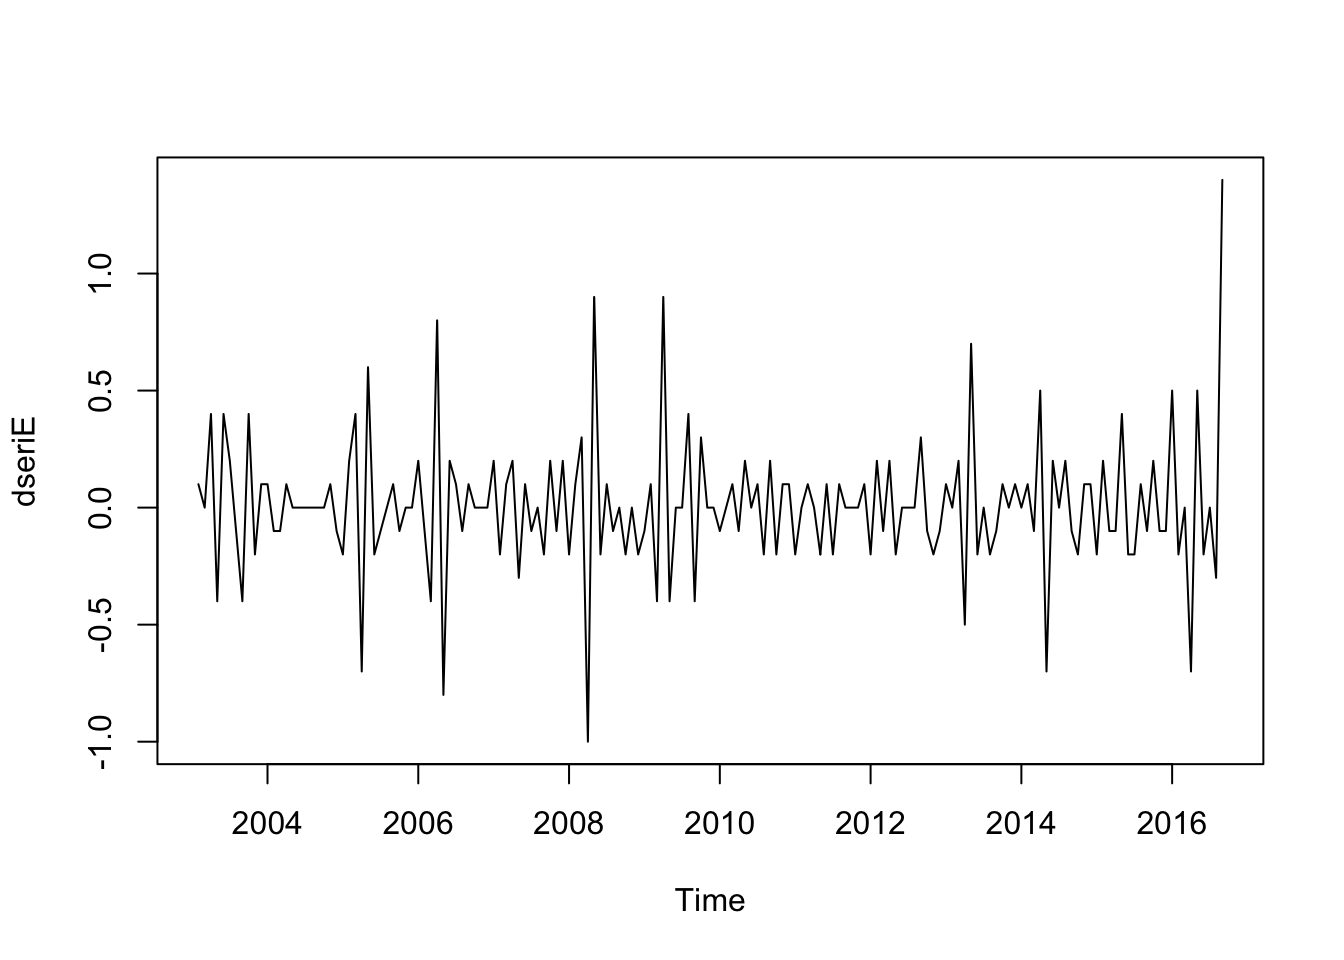
\includegraphics{Julia_Pinol_Touceda_files/figure-latex/unnamed-chunk-4-1.pdf}

A partir del histograma se puede observar que las edades más frecuentes
son las que se encuentran entre los 50 y los 60 años, mientras que las
menos frecuentes van desde los 0 a los 40 y de los 70 a los 80 años. Con
el boxplot y el summary, se puede ver que la edad mínima es de 29 años y
la máxima, de 70.

\textbf{2. Variable sex}

\begin{Shaded}
\begin{Highlighting}[]
\KeywordTok{describe}\NormalTok{(heart}\OperatorTok{$}\NormalTok{sex)}
\end{Highlighting}
\end{Shaded}

\begin{verbatim}
## heart$sex 
##        n  missing distinct 
##      270        0        2 
##                       
## Value          0     1
## Frequency     87   183
## Proportion 0.322 0.678
\end{verbatim}

\begin{Shaded}
\begin{Highlighting}[]
\NormalTok{table_sex <-}\StringTok{ }\KeywordTok{table}\NormalTok{(heart}\OperatorTok{$}\NormalTok{sex)}
\KeywordTok{pie}\NormalTok{(table_sex, }\DataTypeTok{labels =} \KeywordTok{paste}\NormalTok{(}\KeywordTok{c}\NormalTok{(}\StringTok{'0 -'}\NormalTok{, }\StringTok{'1 -'}\NormalTok{), }\KeywordTok{round}\NormalTok{(table_sex}\OperatorTok{/}\DecValTok{270}\NormalTok{,}\DecValTok{2}\NormalTok{)}\OperatorTok{*}\DecValTok{100}\NormalTok{, }\StringTok{'%'}\NormalTok{), }\DataTypeTok{main =} \StringTok{'Diagrama circular de sex'}\NormalTok{,}\DataTypeTok{col=}\KeywordTok{c}\NormalTok{(}\StringTok{'lightblue3'}\NormalTok{,}\StringTok{'lightblue1'}\NormalTok{))}
\end{Highlighting}
\end{Shaded}

\includegraphics{Julia_Pinol_Touceda_files/figure-latex/unnamed-chunk-5-1.pdf}

Se observa que la mayoría de los pacientes son del sexo 1 (68\%) y que
el 32\% son del sexo 2.

\textbf{3. Variable chest\_pain}

\begin{Shaded}
\begin{Highlighting}[]
\KeywordTok{describe}\NormalTok{(heart}\OperatorTok{$}\NormalTok{chest_pain)}
\end{Highlighting}
\end{Shaded}

\begin{verbatim}
## heart$chest_pain 
##        n  missing distinct 
##      270        0        4 
##                                   
## Value          1     2     3     4
## Frequency     20    42    79   129
## Proportion 0.074 0.156 0.293 0.478
\end{verbatim}

\begin{Shaded}
\begin{Highlighting}[]
\NormalTok{table_chpain <-}\StringTok{ }\KeywordTok{table}\NormalTok{(heart}\OperatorTok{$}\NormalTok{chest_pain)}
\KeywordTok{pie}\NormalTok{(table_chpain, }\DataTypeTok{labels =} \KeywordTok{paste}\NormalTok{(}\KeywordTok{c}\NormalTok{(}\StringTok{'Tipo I -'}\NormalTok{, }\StringTok{'Tipo II -'}\NormalTok{, }\StringTok{'Tipo III -'}\NormalTok{, }\StringTok{'Tipo IV -'}\NormalTok{), }\KeywordTok{round}\NormalTok{(table_chpain}\OperatorTok{/}\DecValTok{270}\NormalTok{,}\DecValTok{2}\NormalTok{)}\OperatorTok{*}\DecValTok{100}\NormalTok{, }\StringTok{'%'}\NormalTok{), }\DataTypeTok{main =} \StringTok{'Diagrama circular de chest_pain'}\NormalTok{,}\DataTypeTok{col=}\KeywordTok{c}\NormalTok{(}\StringTok{'lavenderblush'}\NormalTok{,}\StringTok{'lightcyan'}\NormalTok{,}\StringTok{'lightblue1'}\NormalTok{,}\StringTok{'lightblue3'}\NormalTok{))}
\end{Highlighting}
\end{Shaded}

\includegraphics{Julia_Pinol_Touceda_files/figure-latex/unnamed-chunk-6-1.pdf}

En el diagrama de pastel realizado se muestra que un dolor en el pecho
de tipo IV es lo más frecuente, con un 48\% de los casos, seguido de
dolor en el pecho de tipo III, con un 29\%. Menos frecuente es el dolor
tipo II, con un 16\% de los pacientes, y finlmente, el del tipo I, con
un 7\%.

\textbf{4. Variable resting\_BP}

\begin{Shaded}
\begin{Highlighting}[]
\NormalTok{(}\KeywordTok{c}\NormalTok{(}\KeywordTok{summary}\NormalTok{(heart}\OperatorTok{$}\NormalTok{resting_BP),}\DataTypeTok{sd=}\KeywordTok{sd}\NormalTok{(heart}\OperatorTok{$}\NormalTok{resting_BP)))}
\end{Highlighting}
\end{Shaded}

\begin{verbatim}
##      Min.   1st Qu.    Median      Mean   3rd Qu.      Max.        sd 
##  94.00000 120.00000 130.00000 131.30000 140.00000 200.00000  17.86161
\end{verbatim}

\begin{Shaded}
\begin{Highlighting}[]
\KeywordTok{par}\NormalTok{(}\DataTypeTok{mfrow=}\KeywordTok{c}\NormalTok{(}\DecValTok{1}\NormalTok{,}\DecValTok{2}\NormalTok{), }\DataTypeTok{las=}\DecValTok{1}\NormalTok{)}
\KeywordTok{hist}\NormalTok{(heart}\OperatorTok{$}\NormalTok{resting_BP, }\DataTypeTok{ylab =} \StringTok{'Frecuencia'}\NormalTok{, }\DataTypeTok{xlab =} \StringTok{'resting_BP'}\NormalTok{, }\DataTypeTok{main =} \StringTok{'Histograma de resting_BP'}\NormalTok{, }\DataTypeTok{col =} \StringTok{'lightblue3'}\NormalTok{)}
\KeywordTok{boxplot}\NormalTok{(heart}\OperatorTok{$}\NormalTok{resting_BP, }\DataTypeTok{main =} \StringTok{'Boxplot de resting_BP'}\NormalTok{, }\DataTypeTok{col =} \StringTok{'lightblue3'}\NormalTok{)}
\end{Highlighting}
\end{Shaded}

\includegraphics{Julia_Pinol_Touceda_files/figure-latex/unnamed-chunk-7-1.pdf}

Tanto en el hitograma como en el box-plot se puede ver que el valor
medio de la presión de la sangre en reposo está alrededor de 130. Cabe
mencionar también que hay bastantes valores alejados de la media,
sobretodo superiormente.

\textbf{5. Variable serum\_cholest}

\begin{Shaded}
\begin{Highlighting}[]
\NormalTok{(}\KeywordTok{c}\NormalTok{(}\KeywordTok{summary}\NormalTok{(heart}\OperatorTok{$}\NormalTok{serum_cholest),}\DataTypeTok{sd=}\KeywordTok{sd}\NormalTok{(heart}\OperatorTok{$}\NormalTok{serum_cholest)))}
\end{Highlighting}
\end{Shaded}

\begin{verbatim}
##      Min.   1st Qu.    Median      Mean   3rd Qu.      Max.        sd 
## 126.00000 213.00000 245.00000 249.70000 280.00000 564.00000  51.68624
\end{verbatim}

\begin{Shaded}
\begin{Highlighting}[]
\KeywordTok{par}\NormalTok{(}\DataTypeTok{mfrow=}\KeywordTok{c}\NormalTok{(}\DecValTok{1}\NormalTok{,}\DecValTok{2}\NormalTok{), }\DataTypeTok{las=}\DecValTok{1}\NormalTok{)}
\KeywordTok{hist}\NormalTok{(heart}\OperatorTok{$}\NormalTok{serum_cholest, }\DataTypeTok{ylab =} \StringTok{'Frecuencia'}\NormalTok{, }\DataTypeTok{xlab =} \StringTok{'serum_cholest'}\NormalTok{, }\DataTypeTok{main =} \StringTok{'Histograma de serum_cholest'}\NormalTok{, }\DataTypeTok{col =} \StringTok{'lightblue3'}\NormalTok{)}
\KeywordTok{boxplot}\NormalTok{(heart}\OperatorTok{$}\NormalTok{serum_cholest, }\DataTypeTok{col =} \StringTok{'lightblue3'}\NormalTok{, }\DataTypeTok{main =} \StringTok{'Boxplot de serum_cholest'}\NormalTok{)}
\end{Highlighting}
\end{Shaded}

\includegraphics{Julia_Pinol_Touceda_files/figure-latex/unnamed-chunk-8-1.pdf}

Los niveles séricos de colesterol en los pacientes es de media
aproximadamente igual a 250. La mayoría de los pacientes tienen un nivel
sérico alrededor de 200-300 mg/dL. Vemos que la desviación de esta
variable es muy alta, esto se puede deber a que hay varios valores muy
por encima de la media y del tercer cuartil, así como alguno que está
por debajo.

\textbf{6. Variable blood\_sugar}

\begin{Shaded}
\begin{Highlighting}[]
\KeywordTok{describe}\NormalTok{(heart}\OperatorTok{$}\NormalTok{blood_sugar)}
\end{Highlighting}
\end{Shaded}

\begin{verbatim}
## heart$blood_sugar 
##        n  missing distinct 
##      270        0        2 
##                       
## Value          0     1
## Frequency    230    40
## Proportion 0.852 0.148
\end{verbatim}

\begin{Shaded}
\begin{Highlighting}[]
\NormalTok{table_blsugar <-}\StringTok{ }\KeywordTok{table}\NormalTok{(heart}\OperatorTok{$}\NormalTok{blood_sugar)}
\KeywordTok{pie}\NormalTok{(table_blsugar, }\DataTypeTok{labels =} \KeywordTok{paste}\NormalTok{(}\KeywordTok{c}\NormalTok{(}\StringTok{'0 -'}\NormalTok{, }\StringTok{'1 -'}\NormalTok{), }\KeywordTok{round}\NormalTok{(table_blsugar}\OperatorTok{/}\DecValTok{270}\NormalTok{,}\DecValTok{2}\NormalTok{)}\OperatorTok{*}\DecValTok{100}\NormalTok{, }\StringTok{'%'}\NormalTok{), }\DataTypeTok{main =} \StringTok{'Diagrama circular de blood_sugar'}\NormalTok{,}\DataTypeTok{col=}\KeywordTok{c}\NormalTok{(}\StringTok{'lightblue3'}\NormalTok{,}\StringTok{'lightblue1'}\NormalTok{))}
\end{Highlighting}
\end{Shaded}

\includegraphics{Julia_Pinol_Touceda_files/figure-latex/unnamed-chunk-9-1.pdf}

Al rededor de 40 pacientes tienen el nivel de azúcar en la sangre en
ayunas mayor a 120 mg/dL, lo que representa un 15\%, por lo que el 85\%
restante lo tienen inferior a 120.

\textbf{7. Variable electro}

\begin{Shaded}
\begin{Highlighting}[]
\KeywordTok{describe}\NormalTok{(heart}\OperatorTok{$}\NormalTok{electro)}
\end{Highlighting}
\end{Shaded}

\begin{verbatim}
## heart$electro 
##        n  missing distinct 
##      270        0        3 
##                             
## Value          0     1     2
## Frequency    131     2   137
## Proportion 0.485 0.007 0.507
\end{verbatim}

\begin{Shaded}
\begin{Highlighting}[]
\NormalTok{table_electro <-}\StringTok{ }\KeywordTok{table}\NormalTok{(heart}\OperatorTok{$}\NormalTok{electro)}
\KeywordTok{pie}\NormalTok{(table_electro, }\DataTypeTok{labels =} \KeywordTok{paste}\NormalTok{(}\KeywordTok{c}\NormalTok{(}\StringTok{'0 -'}\NormalTok{, }\StringTok{'1 -'}\NormalTok{, }\StringTok{'2 -'}\NormalTok{), }\KeywordTok{round}\NormalTok{(table_electro}\OperatorTok{/}\DecValTok{270}\NormalTok{,}\DecValTok{4}\NormalTok{)}\OperatorTok{*}\DecValTok{100}\NormalTok{, }\StringTok{'%'}\NormalTok{), }\DataTypeTok{main =} \StringTok{'Diagrama circular de electro'}\NormalTok{,}\DataTypeTok{col=}\KeywordTok{c}\NormalTok{(}\StringTok{'lightblue3'}\NormalTok{,}\StringTok{'lavenderblush'}\NormalTok{,}\StringTok{'lightblue1'}\NormalTok{))}
\end{Highlighting}
\end{Shaded}

\includegraphics{Julia_Pinol_Touceda_files/figure-latex/unnamed-chunk-10-1.pdf}

El 48.52\% de los pacientes tienen el nivel 0 en los resultados
electrocardiográficos y el 50.74\% a nivel 2. Menos del 1\% de los
pacientes tienen los resultados electrocardiográficos a nivel 1.

\textbf{8. Variable HR}

\begin{Shaded}
\begin{Highlighting}[]
\NormalTok{(}\KeywordTok{c}\NormalTok{(}\KeywordTok{summary}\NormalTok{(heart}\OperatorTok{$}\NormalTok{HR),}\DataTypeTok{sd=}\KeywordTok{sd}\NormalTok{(heart}\OperatorTok{$}\NormalTok{HR)))}
\end{Highlighting}
\end{Shaded}

\begin{verbatim}
##      Min.   1st Qu.    Median      Mean   3rd Qu.      Max.        sd 
##  71.00000 133.00000 153.50000 149.70000 166.00000 202.00000  23.16572
\end{verbatim}

\begin{Shaded}
\begin{Highlighting}[]
\KeywordTok{par}\NormalTok{(}\DataTypeTok{mfrow=}\KeywordTok{c}\NormalTok{(}\DecValTok{1}\NormalTok{,}\DecValTok{2}\NormalTok{), }\DataTypeTok{las=}\DecValTok{1}\NormalTok{)}
\KeywordTok{hist}\NormalTok{(heart}\OperatorTok{$}\NormalTok{HR, }\DataTypeTok{ylab =} \StringTok{'Frecuencia'}\NormalTok{, }\DataTypeTok{xlab =} \StringTok{'HR'}\NormalTok{, }\DataTypeTok{main =} \StringTok{'Histograma de HR'}\NormalTok{, }\DataTypeTok{col =} \StringTok{'lightblue3'}\NormalTok{)}
\KeywordTok{boxplot}\NormalTok{(heart}\OperatorTok{$}\NormalTok{HR, }\DataTypeTok{main =} \StringTok{'Boxplot de HR'}\NormalTok{, }\DataTypeTok{col =} \StringTok{'lightblue3'}\NormalTok{)}
\end{Highlighting}
\end{Shaded}

\includegraphics{Julia_Pinol_Touceda_files/figure-latex/unnamed-chunk-11-1.pdf}

Vemos que la media de HR está alrededor de 150, siendo los cuartiles
primero y tercero aproximadamente del 133 y 167 \%. Sin embargo el valor
máximo es de 202 y el mínimo de 71. Estos valores alejados de la media
hacen que la variabilidad sea alta.

\textbf{9. Varible exercise}

\begin{Shaded}
\begin{Highlighting}[]
\KeywordTok{describe}\NormalTok{(heart}\OperatorTok{$}\NormalTok{exercise)}
\end{Highlighting}
\end{Shaded}

\begin{verbatim}
## heart$exercise 
##        n  missing distinct 
##      270        0        2 
##                     
## Value         0    1
## Frequency   181   89
## Proportion 0.67 0.33
\end{verbatim}

\begin{Shaded}
\begin{Highlighting}[]
\NormalTok{table_exercise <-}\StringTok{ }\KeywordTok{table}\NormalTok{(heart}\OperatorTok{$}\NormalTok{exercise)}
\KeywordTok{pie}\NormalTok{(table_exercise, }\DataTypeTok{labels =} \KeywordTok{paste}\NormalTok{(}\KeywordTok{c}\NormalTok{(}\StringTok{'0 -'}\NormalTok{, }\StringTok{'1 -'}\NormalTok{), }\KeywordTok{round}\NormalTok{(table_exercise}\OperatorTok{/}\DecValTok{270}\NormalTok{,}\DecValTok{2}\NormalTok{)}\OperatorTok{*}\DecValTok{100}\NormalTok{, }\StringTok{'%'}\NormalTok{), }\DataTypeTok{main =} \StringTok{'Diagrama circular de exercise'}\NormalTok{,}\DataTypeTok{col=}\KeywordTok{c}\NormalTok{(}\StringTok{'lightblue3'}\NormalTok{,}\StringTok{'lightblue1'}\NormalTok{))}
\end{Highlighting}
\end{Shaded}

\includegraphics{Julia_Pinol_Touceda_files/figure-latex/unnamed-chunk-12-1.pdf}

Con el diagrama de pastel anterior se puede ver como a la mayoría de
pacientes (67\%) el ejercicio no le indujo la angina, mientas que al
33\% de los pacientes sí.

\textbf{10. Variable oldpeak}

\begin{Shaded}
\begin{Highlighting}[]
\NormalTok{(}\KeywordTok{c}\NormalTok{(}\KeywordTok{summary}\NormalTok{(heart}\OperatorTok{$}\NormalTok{oldpeak),}\DataTypeTok{sd=}\KeywordTok{sd}\NormalTok{(heart}\OperatorTok{$}\NormalTok{oldpeak)))}
\end{Highlighting}
\end{Shaded}

\begin{verbatim}
##    Min. 1st Qu.  Median    Mean 3rd Qu.    Max.      sd 
## 0.00000 0.00000 0.80000 1.05000 1.60000 6.20000 1.14521
\end{verbatim}

\begin{Shaded}
\begin{Highlighting}[]
\KeywordTok{par}\NormalTok{(}\DataTypeTok{mfrow=}\KeywordTok{c}\NormalTok{(}\DecValTok{1}\NormalTok{,}\DecValTok{2}\NormalTok{), }\DataTypeTok{las=}\DecValTok{1}\NormalTok{)}
\KeywordTok{hist}\NormalTok{(heart}\OperatorTok{$}\NormalTok{oldpeak, }\DataTypeTok{ylab =} \StringTok{'Frecuencia'}\NormalTok{, }\DataTypeTok{xlab =} \StringTok{'oldpeak'}\NormalTok{, }\DataTypeTok{main =} \StringTok{'Histograma de oldpeak'}\NormalTok{, }\DataTypeTok{col =} \StringTok{'lightblue3'}\NormalTok{)}
\KeywordTok{boxplot}\NormalTok{(heart}\OperatorTok{$}\NormalTok{oldpeak, }\DataTypeTok{main =} \StringTok{'Boxplot de oldpeak'}\NormalTok{, }\DataTypeTok{col =} \StringTok{'lightblue3'}\NormalTok{)}
\end{Highlighting}
\end{Shaded}

\includegraphics{Julia_Pinol_Touceda_files/figure-latex/unnamed-chunk-13-1.pdf}

Esta variable indica si a los pacientes les han tenido que inducir
depresion ST a través del ejercicio en relación con el descanso.

Los valores de oldpeak tienen una media igual a 1.05, su valor máximo es
de 6.2 estando este muy alejado de la media y del tercer cuartil. Con
ambos gráficos se observa cómo la variable oldpeak tiene una
distribución asimétrica positiva, es decir, hay muchos valores enre el 0
i el 3 y muy pocos del 2 al 6.

\textbf{11. Variable ST}

\begin{Shaded}
\begin{Highlighting}[]
\KeywordTok{describe}\NormalTok{(heart}\OperatorTok{$}\NormalTok{ST)}
\end{Highlighting}
\end{Shaded}

\begin{verbatim}
## heart$ST 
##        n  missing distinct 
##      270        0        3 
##                             
## Value          1     2     3
## Frequency    130   122    18
## Proportion 0.481 0.452 0.067
\end{verbatim}

\begin{Shaded}
\begin{Highlighting}[]
\NormalTok{table_ST <-}\StringTok{ }\KeywordTok{table}\NormalTok{(heart}\OperatorTok{$}\NormalTok{ST)}
\KeywordTok{pie}\NormalTok{(table_ST, }\DataTypeTok{labels =} \KeywordTok{paste}\NormalTok{(}\KeywordTok{c}\NormalTok{(}\StringTok{'1 -'}\NormalTok{, }\StringTok{'2 -'}\NormalTok{, }\StringTok{'3 -'}\NormalTok{), }\KeywordTok{round}\NormalTok{(table_ST}\OperatorTok{/}\DecValTok{270}\NormalTok{,}\DecValTok{2}\NormalTok{)}\OperatorTok{*}\DecValTok{100}\NormalTok{, }\StringTok{'%'}\NormalTok{), }\DataTypeTok{main =} \StringTok{'Diagrama circular de ST'}\NormalTok{,}\DataTypeTok{col=}\KeywordTok{c}\NormalTok{(}\StringTok{'lightblue3'}\NormalTok{,}\StringTok{'lightblue1'}\NormalTok{,}\StringTok{'lavenderblush'}\NormalTok{))}
\end{Highlighting}
\end{Shaded}

\includegraphics{Julia_Pinol_Touceda_files/figure-latex/unnamed-chunk-14-1.pdf}

Se puede ver que la opción 1 y 2 son las más abundantes, suponiendo
entre las dos a casi el 94\% de la totalidad de las respuestas.

\textbf{12. Variable major\_vessels}

\begin{Shaded}
\begin{Highlighting}[]
\KeywordTok{describe}\NormalTok{(heart}\OperatorTok{$}\NormalTok{major_vessels)}
\end{Highlighting}
\end{Shaded}

\begin{verbatim}
## heart$major_vessels 
##        n  missing distinct 
##      270        0        4 
##                                   
## Value          0     1     2     3
## Frequency    160    58    33    19
## Proportion 0.593 0.215 0.122 0.070
\end{verbatim}

\begin{Shaded}
\begin{Highlighting}[]
\NormalTok{table_mjvessels <-}\StringTok{ }\KeywordTok{table}\NormalTok{(heart}\OperatorTok{$}\NormalTok{major_vessels)}
\KeywordTok{pie}\NormalTok{(table_mjvessels, }\DataTypeTok{labels =} \KeywordTok{paste}\NormalTok{(}\KeywordTok{c}\NormalTok{(}\StringTok{'0 -'}\NormalTok{, }\StringTok{'1 -'}\NormalTok{, }\StringTok{'2 -'}\NormalTok{,}\StringTok{'3 -'}\NormalTok{), }\KeywordTok{round}\NormalTok{(table_mjvessels}\OperatorTok{/}\DecValTok{270}\NormalTok{,}\DecValTok{2}\NormalTok{)}\OperatorTok{*}\DecValTok{100}\NormalTok{, }\StringTok{'%'}\NormalTok{), }\DataTypeTok{main =} \StringTok{'Diagrama circular de major_vessels'}\NormalTok{,}\DataTypeTok{col=}\KeywordTok{c}\NormalTok{(}\StringTok{'lightblue3'}\NormalTok{,}\StringTok{'lightblue1'}\NormalTok{,}\StringTok{'lavenderblush'}\NormalTok{,}\StringTok{'lightcyan'}\NormalTok{))}
\end{Highlighting}
\end{Shaded}

\includegraphics{Julia_Pinol_Touceda_files/figure-latex/unnamed-chunk-15-1.pdf}

En este caso vemos que lo más común es que ningún vaso haya sido
coloreado por fluoroscopia, suponiendo casi un 60\% de las observaciones
totales. Mientras que lo menos común es que los 3 vasos lo hayan sido,
suponiendo sólo un 7\% de las observaciones totales.

\textbf{13. Variable thal}

\begin{Shaded}
\begin{Highlighting}[]
\KeywordTok{describe}\NormalTok{(heart}\OperatorTok{$}\NormalTok{thal)}
\end{Highlighting}
\end{Shaded}

\begin{verbatim}
## heart$thal 
##        n  missing distinct 
##      270        0        3 
##                             
## Value          3     6     7
## Frequency    152    14   104
## Proportion 0.563 0.052 0.385
\end{verbatim}

\begin{Shaded}
\begin{Highlighting}[]
\NormalTok{table_thal <-}\StringTok{ }\KeywordTok{table}\NormalTok{(heart}\OperatorTok{$}\NormalTok{thal)}
\KeywordTok{pie}\NormalTok{(table_thal, }\DataTypeTok{labels =} \KeywordTok{paste}\NormalTok{(}\KeywordTok{c}\NormalTok{(}\StringTok{'normal'}\NormalTok{, }\StringTok{'fixed defect'}\NormalTok{, }\StringTok{'reversable defect'}\NormalTok{), }\KeywordTok{round}\NormalTok{(table_thal}\OperatorTok{/}\DecValTok{270}\NormalTok{,}\DecValTok{2}\NormalTok{)}\OperatorTok{*}\DecValTok{100}\NormalTok{, }\StringTok{'%'}\NormalTok{), }\DataTypeTok{main =} \StringTok{'Diagrama circular de thal'}\NormalTok{,}\DataTypeTok{col=}\KeywordTok{c}\NormalTok{(}\StringTok{'lightblue3'}\NormalTok{,}\StringTok{'lavenderblush'}\NormalTok{,}\StringTok{'lightblue1'}\NormalTok{,}\StringTok{'lightcyan'}\NormalTok{))}
\end{Highlighting}
\end{Shaded}

\includegraphics{Julia_Pinol_Touceda_files/figure-latex/unnamed-chunk-16-1.pdf}

El 56\% de los pacientes tienen un thal normal, el 39\% un defecto
reversible mientras que tan solo el 5\% muestra un defecto fijo.

\textbf{14. Variable disease}

\begin{Shaded}
\begin{Highlighting}[]
\KeywordTok{describe}\NormalTok{(heart}\OperatorTok{$}\NormalTok{disease)}
\end{Highlighting}
\end{Shaded}

\begin{verbatim}
## heart$disease 
##        n  missing distinct 
##      270        0        2 
##                       
## Value          1     2
## Frequency    150   120
## Proportion 0.556 0.444
\end{verbatim}

\begin{Shaded}
\begin{Highlighting}[]
\NormalTok{(table_disease <-}\StringTok{ }\KeywordTok{table}\NormalTok{(heart}\OperatorTok{$}\NormalTok{disease))}
\end{Highlighting}
\end{Shaded}

\begin{verbatim}
## 
##   1   2 
## 150 120
\end{verbatim}

\begin{Shaded}
\begin{Highlighting}[]
\KeywordTok{pie}\NormalTok{(table_disease, }\DataTypeTok{labels =} \KeywordTok{paste}\NormalTok{(}\KeywordTok{c}\NormalTok{(}\StringTok{'Absence'}\NormalTok{, }\StringTok{'Presence'}\NormalTok{), }\KeywordTok{round}\NormalTok{(table_disease}\OperatorTok{/}\DecValTok{270}\NormalTok{,}\DecValTok{2}\NormalTok{)}\OperatorTok{*}\DecValTok{100}\NormalTok{, }\StringTok{'%'}\NormalTok{), }\DataTypeTok{main =} \StringTok{'Diagrama circular de table_disease'}\NormalTok{,}\DataTypeTok{col=}\KeywordTok{c}\NormalTok{(}\StringTok{'lightblue3'}\NormalTok{,}\StringTok{'lightblue1'}\NormalTok{))}
\end{Highlighting}
\end{Shaded}

\includegraphics{Julia_Pinol_Touceda_files/figure-latex/unnamed-chunk-17-1.pdf}

El 56\% de los pacientes estudiados no sufren esta enfermedad coronaria
frente a un 44\% que sí la sufren.

\subsection{1.2. Descriptiva bivariante entre las predictoras y la
respuesta.}\label{descriptiva-bivariante-entre-las-predictoras-y-la-respuesta.}

\begin{Shaded}
\begin{Highlighting}[]
\NormalTok{vars=}\KeywordTok{colnames}\NormalTok{(heart)[}\OperatorTok{-}\DecValTok{14}\NormalTok{]}
\KeywordTok{par}\NormalTok{(}\DataTypeTok{mfrow=}\KeywordTok{c}\NormalTok{(}\DecValTok{4}\NormalTok{,}\DecValTok{5}\NormalTok{),}\DataTypeTok{mar=}\KeywordTok{c}\NormalTok{(}\DecValTok{3}\NormalTok{,}\DecValTok{3}\NormalTok{,}\DecValTok{3}\NormalTok{,}\DecValTok{1}\NormalTok{))}
\ControlFlowTok{for}\NormalTok{ (va }\ControlFlowTok{in}\NormalTok{ vars)\{}
  \ControlFlowTok{if}\NormalTok{ (}\OperatorTok{!}\KeywordTok{is.factor}\NormalTok{(heart[,va]))\{}
    \KeywordTok{boxplot}\NormalTok{(}\KeywordTok{as.formula}\NormalTok{(}\KeywordTok{paste0}\NormalTok{(va,}\StringTok{"~disease"}\NormalTok{)),heart,}\DataTypeTok{main=}\NormalTok{va,}\DataTypeTok{col=}\KeywordTok{c}\NormalTok{(}\StringTok{'lightblue3'}\NormalTok{,}\StringTok{'lightblue1'}\NormalTok{),}\DataTypeTok{horizontal=}\NormalTok{T)}
\NormalTok{  \} }\ControlFlowTok{else}\NormalTok{\{}
    \KeywordTok{plot}\NormalTok{(}\KeywordTok{as.formula}\NormalTok{(}\KeywordTok{paste0}\NormalTok{(}\StringTok{"disease~"}\NormalTok{,va)),heart,}\DataTypeTok{main=}\NormalTok{va,}\DataTypeTok{col=}\KeywordTok{c}\NormalTok{(}\StringTok{'lightblue3'}\NormalTok{,}\StringTok{'lightblue1'}\NormalTok{))}
\NormalTok{  \}}
\NormalTok{\}}
\end{Highlighting}
\end{Shaded}

\includegraphics{Julia_Pinol_Touceda_files/figure-latex/unnamed-chunk-18-1.pdf}

A continuación se realizará una descriptiva bivariante entre la variable
respuesta (disease) y las variables que en el apartado anterior parecen
cambiar más en función del valor de la variable respuesta disease.

\textbf{1. Variables disease y Sex}

\begin{Shaded}
\begin{Highlighting}[]
\CommentTok{#install.packages("catspec")}
\KeywordTok{library}\NormalTok{(catspec)}
\KeywordTok{levels}\NormalTok{(heart}\OperatorTok{$}\NormalTok{disease)<-}\KeywordTok{c}\NormalTok{(}\StringTok{'No padece'}\NormalTok{,}\StringTok{'Si padece'}\NormalTok{)}
\KeywordTok{with}\NormalTok{(heart,}\KeywordTok{table}\NormalTok{(sex,disease)) }
\end{Highlighting}
\end{Shaded}

\begin{verbatim}
##    disease
## sex No padece Si padece
##   0        67        20
##   1        83       100
\end{verbatim}

\begin{Shaded}
\begin{Highlighting}[]
\KeywordTok{ctab}\NormalTok{(heart}\OperatorTok{$}\NormalTok{sex,heart}\OperatorTok{$}\NormalTok{disease,}\DataTypeTok{type=}\KeywordTok{c}\NormalTok{(}\StringTok{"n"}\NormalTok{,}\StringTok{"r"}\NormalTok{,}\StringTok{"t"}\NormalTok{,}\StringTok{"r"}\NormalTok{),}\DataTypeTok{addmargins=}\NormalTok{T)}
\end{Highlighting}
\end{Shaded}

\begin{verbatim}
##              Var2 No padece Si padece    Sum
## Var1                                        
## 0    Count            67.00     20.00  87.00
##      Row %            77.01     22.99 100.00
##      Total %          24.81      7.41  32.22
##      row              77.01     22.99 100.00
## 1    Count            83.00    100.00 183.00
##      Row %            45.36     54.64 100.00
##      Total %          30.74     37.04  67.78
##      row              45.36     54.64 100.00
## Sum  Count           150.00    120.00 270.00
##      Row %           122.37     77.63 200.00
##      Total %          55.56     44.44 100.00
##      row             122.37     77.63 200.00
\end{verbatim}

Vemos que no hay gran diferencia en función del sexo en cuanto a que no
padecen la enfermedad. Sin embargo, vemos que si parece haber relación
entre el sexo y el hecho de sí padecer una enfermedad de corazón.

\textbf{2. Variables disease y Edad}

\begin{Shaded}
\begin{Highlighting}[]
\KeywordTok{with}\NormalTok{(heart,}\KeywordTok{tapply}\NormalTok{(age,disease,summary)) }
\end{Highlighting}
\end{Shaded}

\begin{verbatim}
## $`No padece`
##    Min. 1st Qu.  Median    Mean 3rd Qu.    Max. 
##   29.00   45.00   52.00   52.71   59.00   76.00 
## 
## $`Si padece`
##    Min. 1st Qu.  Median    Mean 3rd Qu.    Max. 
##   35.00   52.00   58.00   56.59   62.00   77.00
\end{verbatim}

\begin{Shaded}
\begin{Highlighting}[]
\KeywordTok{boxplot}\NormalTok{(age}\OperatorTok{~}\NormalTok{disease,}\DataTypeTok{data=}\NormalTok{heart,}\DataTypeTok{col=}\KeywordTok{c}\NormalTok{(}\StringTok{'lightblue3'}\NormalTok{,}\StringTok{'lightblue1'}\NormalTok{))}
\end{Highlighting}
\end{Shaded}

\includegraphics{Julia_Pinol_Touceda_files/figure-latex/unnamed-chunk-20-1.pdf}

Se puede ver cómo aquellos pacientes que si presentaron la enfermedad
tienen una media de edad 4 años superior al grupo de pacientes que no la
han padecido. En ambos casos la edad máxima es similar (77 y 76 años).

\textbf{3. Variables disease y Chest pain}

\begin{Shaded}
\begin{Highlighting}[]
\KeywordTok{with}\NormalTok{(heart,}\KeywordTok{table}\NormalTok{(chest_pain,disease)) }
\end{Highlighting}
\end{Shaded}

\begin{verbatim}
##           disease
## chest_pain No padece Si padece
##          1        15         5
##          2        35         7
##          3        62        17
##          4        38        91
\end{verbatim}

\begin{Shaded}
\begin{Highlighting}[]
\KeywordTok{ctab}\NormalTok{(heart}\OperatorTok{$}\NormalTok{chest_pain,heart}\OperatorTok{$}\NormalTok{disease,}\DataTypeTok{type=}\KeywordTok{c}\NormalTok{(}\StringTok{"n"}\NormalTok{,}\StringTok{"r"}\NormalTok{,}\StringTok{"t"}\NormalTok{,}\StringTok{"r"}\NormalTok{),}\DataTypeTok{addmargins=}\NormalTok{T)}
\end{Highlighting}
\end{Shaded}

\begin{verbatim}
##              Var2 No padece Si padece    Sum
## Var1                                        
## 1    Count            15.00      5.00  20.00
##      Row %            75.00     25.00 100.00
##      Total %           5.56      1.85   7.41
##      row              75.00     25.00 100.00
## 2    Count            35.00      7.00  42.00
##      Row %            83.33     16.67 100.00
##      Total %          12.96      2.59  15.56
##      row              83.33     16.67 100.00
## 3    Count            62.00     17.00  79.00
##      Row %            78.48     21.52 100.00
##      Total %          22.96      6.30  29.26
##      row              78.48     21.52 100.00
## 4    Count            38.00     91.00 129.00
##      Row %            29.46     70.54 100.00
##      Total %          14.07     33.70  47.78
##      row              29.46     70.54 100.00
## Sum  Count           150.00    120.00 270.00
##      Row %           266.27    133.73 400.00
##      Total %          55.56     44.44 100.00
##      row             266.27    133.73 400.00
\end{verbatim}

\begin{Shaded}
\begin{Highlighting}[]
\KeywordTok{plot}\NormalTok{(disease}\OperatorTok{~}\NormalTok{chest_pain,}\DataTypeTok{data=}\NormalTok{heart,}\DataTypeTok{col=}\KeywordTok{c}\NormalTok{(}\StringTok{'lightblue3'}\NormalTok{,}\StringTok{'lightblue1'}\NormalTok{))}
\end{Highlighting}
\end{Shaded}

\includegraphics{Julia_Pinol_Touceda_files/figure-latex/unnamed-chunk-21-1.pdf}

Con el plot anterior se observa que los pacientes que padecen
enfermedades coronárias muestran un dolor de pecho tipo 4 esto es, el
70\% de los pacientes.

\textbf{4. Variables disease y Exercice}

\begin{Shaded}
\begin{Highlighting}[]
\KeywordTok{with}\NormalTok{(heart,}\KeywordTok{table}\NormalTok{(exercise,disease)) }
\end{Highlighting}
\end{Shaded}

\begin{verbatim}
##         disease
## exercise No padece Si padece
##        0       127        54
##        1        23        66
\end{verbatim}

\begin{Shaded}
\begin{Highlighting}[]
\KeywordTok{plot}\NormalTok{(disease}\OperatorTok{~}\NormalTok{exercise,}\DataTypeTok{data=}\NormalTok{heart,}\DataTypeTok{col=}\KeywordTok{c}\NormalTok{(}\StringTok{'lightblue3'}\NormalTok{,}\StringTok{'lightblue1'}\NormalTok{))}
\end{Highlighting}
\end{Shaded}

\includegraphics{Julia_Pinol_Touceda_files/figure-latex/unnamed-chunk-22-1.pdf}

Existe una gran diferencia entre los individuos que realizan ejericio
tipo 0 de los que realizan de tipo 1. La proporcion de individuos que
padecen la enfermedad es mucho menor en los del primer tipo (54
pacientes de los 120 que presentan enfermedades de corazón frente a
66/120).

\textbf{5. Variables disease y Oldpeak}

\begin{Shaded}
\begin{Highlighting}[]
\KeywordTok{with}\NormalTok{(heart,}\KeywordTok{tapply}\NormalTok{(oldpeak,disease,summary)) }
\end{Highlighting}
\end{Shaded}

\begin{verbatim}
## $`No padece`
##    Min. 1st Qu.  Median    Mean 3rd Qu.    Max. 
##  0.0000  0.0000  0.2000  0.6227  1.1750  4.2000 
## 
## $`Si padece`
##    Min. 1st Qu.  Median    Mean 3rd Qu.    Max. 
##   0.000   0.600   1.400   1.584   2.425   6.200
\end{verbatim}

Las personas que padecen enfermedades de corazón tienen un mayor nivel
de oldpeak; tienen una mediana 1.2 puntos superior y también el valor
máximo es bastante superior (2 puntos).

\textbf{6. Variables disease y ST}

\begin{Shaded}
\begin{Highlighting}[]
\KeywordTok{with}\NormalTok{(heart,}\KeywordTok{table}\NormalTok{(ST,disease)) }
\end{Highlighting}
\end{Shaded}

\begin{verbatim}
##    disease
## ST  No padece Si padece
##   1        98        32
##   2        44        78
##   3         8        10
\end{verbatim}

\begin{Shaded}
\begin{Highlighting}[]
\KeywordTok{plot}\NormalTok{(disease}\OperatorTok{~}\NormalTok{ST,}\DataTypeTok{data=}\NormalTok{heart,}\DataTypeTok{col=}\KeywordTok{c}\NormalTok{(}\StringTok{'lightblue3'}\NormalTok{,}\StringTok{'lightblue1'}\NormalTok{))}
\end{Highlighting}
\end{Shaded}

\includegraphics{Julia_Pinol_Touceda_files/figure-latex/unnamed-chunk-24-1.pdf}

Vemos que entre las personas que sí padecen enfermedades de corazón es
más frecuente tener el nivel de ST igual a 2, seguido de 3. De la misma
manera, entre las personas que no las padecen lo más frecuente es tener
el nivel de ST igual a 1.

\textbf{7. Variables disease y Major\_vessels}

\begin{Shaded}
\begin{Highlighting}[]
\KeywordTok{with}\NormalTok{(heart,}\KeywordTok{table}\NormalTok{(major_vessels,disease)) }
\end{Highlighting}
\end{Shaded}

\begin{verbatim}
##              disease
## major_vessels No padece Si padece
##             0       120        40
##             1        20        38
##             2         7        26
##             3         3        16
\end{verbatim}

\begin{Shaded}
\begin{Highlighting}[]
\KeywordTok{plot}\NormalTok{(disease}\OperatorTok{~}\NormalTok{major_vessels,}\DataTypeTok{data=}\NormalTok{heart,}\DataTypeTok{col=}\KeywordTok{c}\NormalTok{(}\StringTok{'lightblue3'}\NormalTok{,}\StringTok{'lightblue1'}\NormalTok{))}
\end{Highlighting}
\end{Shaded}

\includegraphics{Julia_Pinol_Touceda_files/figure-latex/unnamed-chunk-25-1.pdf}

Entre las personas que no padecen la enfermedad es frecuente que ningún
vaso principal haya sido coloreado por fluoroscopia. Sin embargo, entre
las personas que sí padecen éstas enfermedades no se observan grandes
diferencias entre cuantos vasos han sido coloreados, aunque lo menos
frencuente es que hayan sido los 3.

\textbf{8. Variables disease y Thal}

\begin{Shaded}
\begin{Highlighting}[]
\KeywordTok{with}\NormalTok{(heart,}\KeywordTok{table}\NormalTok{(thal,disease)) }
\end{Highlighting}
\end{Shaded}

\begin{verbatim}
##     disease
## thal No padece Si padece
##    3       119        33
##    6         6         8
##    7        25        79
\end{verbatim}

\begin{Shaded}
\begin{Highlighting}[]
\KeywordTok{plot}\NormalTok{(disease}\OperatorTok{~}\NormalTok{thal,}\DataTypeTok{data=}\NormalTok{heart,}\DataTypeTok{col=}\KeywordTok{c}\NormalTok{(}\StringTok{'lightblue3'}\NormalTok{,}\StringTok{'lightblue1'}\NormalTok{))}
\end{Highlighting}
\end{Shaded}

\includegraphics{Julia_Pinol_Touceda_files/figure-latex/unnamed-chunk-26-1.pdf}

Los tipos de thal de defecto reversible (7) o defecto fijo (6) tienen
más pacientes que sí padecen enfermedades de corazón que los que tienen
un tipo de thal normal(3).

\textbf{análisis con ``catdes''}

\begin{Shaded}
\begin{Highlighting}[]
\NormalTok{heart}\OperatorTok{$}\NormalTok{disease <-}\StringTok{ }\KeywordTok{as.factor}\NormalTok{(heart}\OperatorTok{$}\NormalTok{disease)}
\KeywordTok{summary}\NormalTok{(heart}\OperatorTok{$}\NormalTok{disease)}
\end{Highlighting}
\end{Shaded}

\begin{verbatim}
## No padece Si padece 
##       150       120
\end{verbatim}

\begin{Shaded}
\begin{Highlighting}[]
\KeywordTok{levels}\NormalTok{(heart}\OperatorTok{$}\NormalTok{disease) <-}\StringTok{ }\KeywordTok{c}\NormalTok{(}\StringTok{"No padece"}\NormalTok{, }\StringTok{"Si padece"}\NormalTok{)}
\KeywordTok{catdes}\NormalTok{(heart,}\DecValTok{14}\NormalTok{) }\CommentTok{#package FactoMineR}
\end{Highlighting}
\end{Shaded}

\begin{verbatim}
## 
## Link between the cluster variable and the categorical variables (chi-square test)
## =================================================================================
##                    p.value df
## thal          6.419071e-17  2
## chest_pain    8.560988e-15  3
## major_vessels 1.436620e-13  3
## exercise      5.585260e-12  1
## ST            1.712699e-09  2
## sex           9.979047e-07  1
## electro       1.122372e-02  2
## 
## Description of each cluster by the categories
## =============================================
## $`No padece`
##                  Cla/Mod   Mod/Cla    Global      p.value    v.test
## thal=3          78.28947 79.333333 56.296296 5.093470e-18  8.651258
## major_vessels=0 75.00000 80.000000 59.259259 5.289157e-15  7.819838
## exercise=0      70.16575 84.666667 67.037037 4.691873e-12  6.914599
## ST=1            75.38462 65.333333 48.148148 1.960579e-10  6.364397
## sex=0           77.01149 44.666667 32.222222 7.246827e-07  4.954629
## chest_pain=3    78.48101 41.333333 29.259259 7.257472e-07  4.954344
## chest_pain=2    83.33333 23.333333 15.555556 5.115197e-05  4.050300
## electro=0       64.88550 56.666667 48.518519 2.866014e-03  2.981755
## electro=2       46.71533 42.666667 50.740741 3.147375e-03 -2.952965
## major_vessels=3 15.78947  2.000000  7.037037 3.214702e-04 -3.597355
## major_vessels=1 34.48276 13.333333 21.481481 3.089872e-04 -3.607646
## major_vessels=2 21.21212  4.666667 12.222222 2.422890e-05 -4.221865
## sex=1           45.35519 55.333333 67.777778 7.246827e-07 -4.954629
## ST=2            36.06557 29.333333 45.185185 4.621153e-09 -5.860270
## exercise=1      25.84270 15.333333 32.962963 4.691873e-12 -6.914599
## thal=7          24.03846 16.666667 38.518519 7.451161e-17 -8.339649
## chest_pain=4    29.45736 25.333333 47.777778 5.417989e-17 -8.377247
## 
## $`Si padece`
##                  Cla/Mod   Mod/Cla    Global      p.value    v.test
## chest_pain=4    70.54264 75.833333 47.777778 5.417989e-17  8.377247
## thal=7          75.96154 65.833333 38.518519 7.451161e-17  8.339649
## exercise=1      74.15730 55.000000 32.962963 4.691873e-12  6.914599
## ST=2            63.93443 65.000000 45.185185 4.621153e-09  5.860270
## sex=1           54.64481 83.333333 67.777778 7.246827e-07  4.954629
## major_vessels=2 78.78788 21.666667 12.222222 2.422890e-05  4.221865
## major_vessels=1 65.51724 31.666667 21.481481 3.089872e-04  3.607646
## major_vessels=3 84.21053 13.333333  7.037037 3.214702e-04  3.597355
## electro=2       53.28467 60.833333 50.740741 3.147375e-03  2.952965
## electro=0       35.11450 38.333333 48.518519 2.866014e-03 -2.981755
## chest_pain=2    16.66667  5.833333 15.555556 5.115197e-05 -4.050300
## chest_pain=3    21.51899 14.166667 29.259259 7.257472e-07 -4.954344
## sex=0           22.98851 16.666667 32.222222 7.246827e-07 -4.954629
## ST=1            24.61538 26.666667 48.148148 1.960579e-10 -6.364397
## exercise=0      29.83425 45.000000 67.037037 4.691873e-12 -6.914599
## major_vessels=0 25.00000 33.333333 59.259259 5.289157e-15 -7.819838
## thal=3          21.71053 27.500000 56.296296 5.093470e-18 -8.651258
## 
## 
## Link between the cluster variable and the quantitative variables
## ================================================================
##                  Eta2      P-value
## HR         0.17515394 7.119583e-13
## oldpeak    0.17469678 7.677946e-13
## age        0.04508071 4.434804e-04
## resting_BP 0.02414377 1.056095e-02
## 
## Description of each cluster by quantitative variables
## =====================================================
## $`No padece`
##               v.test Mean in category Overall mean sd in category
## HR          6.864139      158.3333333    149.67778     19.2189721
## resting_BP -2.548465      128.8666667    131.34444     16.4027098
## age        -3.482343       52.7066667     54.43333      9.4780776
## oldpeak    -6.855176        0.6226667      1.05000      0.7981768
##            Overall sd      p.value
## HR          23.122778 6.689329e-12
## resting_BP  17.828501 1.081981e-02
## age          9.092182 4.970470e-04
## oldpeak      1.143087 7.122494e-12
## 
## $`Si padece`
##               v.test Mean in category Overall mean sd in category
## oldpeak     6.855176         1.584167      1.05000       1.276714
## age         3.482343        56.591667     54.43333       8.082384
## resting_BP  2.548465       134.441667    131.34444      19.015693
## HR         -6.864139       138.858333    149.67778      23.034140
##            Overall sd      p.value
## oldpeak      1.143087 7.122494e-12
## age          9.092182 4.970470e-04
## resting_BP  17.828501 1.081981e-02
## HR          23.122778 6.689329e-12
\end{verbatim}

La primeras 3 variables categóricas más vinculadas a disease son thal,
seguida de chest\_pain y major\_vessels.

Miramos ahora las dos subpoblaciones correspondientes a los pacientes
que no padecen enfermedades de corazón y los que sí.

La categoría 3 de la variable `thal' así como la categoría 7 de
`major\_vessels' están sobre representadas (v-test \textgreater{}0)
entre las personas que no padecen enfermedades de corazón, en cambio
están subrepresentadas en aquellas personas que sí las padecen.

En cambio, las categorías 4 y 7 de las variables `chest\_pain' y `thal'
respectivamente están sobre representadas en las personas que sí las
padecen mientras que están subrepresentadas en las que no.

Para el subgrupo de personas que sí padecen enfermedades de corazón:

\begin{itemize}
\item
  70,54\% de los individuos que poseen `chest\_pain=4' poseen
  enfermedades de corazón.
\item
  75,83\% de los individuos que poseen enfermedades de corazón poseen
  `chest\_pain=4'
\item
  47,7\% de toda la población posee `chest\_pain=4'
\item
  75,96\% de los individuos que poseen `thal=7' poseen enfermedades de
  corazón.
\item
  65,833\% de los individuos que poseen enfermedades de corazón poseen
  `thal=7'
\item
  38,52\% de toda la población posee `thal=7'
\end{itemize}

Para el caso de las variables continuas vemos que hay 4 que están
significativamente relacionadas con el hecho de padecer o no
enfermedades de corazón, estas variables son : oldpeak, age,
resting\_BP, HR

\section{2. Depuración de datos.}\label{depuracion-de-datos.}

La variable disease estaba categorizada como `1'\{no padece\} y `2'\{si
padece\}, por lo que para la descriptiva hemos cambiado los niveles a
los que aparecen entre corchetes. Para los siguientes puntos hemos
creado una nueva variable ``resp'' que toma los valores `0' y `1'.

En primer lugar, agrupamos los 3 primeros niveles de chest\_pain en un
mismo nivel, que en este caso es 0. Por otro lado, dejamos el nivel 4
que es el único que aparece muy vinculado con el hecho de padecer este
tipo de enfermedad.

\begin{Shaded}
\begin{Highlighting}[]
\NormalTok{heart}\OperatorTok{$}\NormalTok{chest_pain4[heart}\OperatorTok{$}\NormalTok{chest_pain }\OperatorTok{==}\StringTok{ }\DecValTok{4}\NormalTok{] <-}\StringTok{ '4'}
\NormalTok{heart}\OperatorTok{$}\NormalTok{chest_pain4[heart}\OperatorTok{$}\NormalTok{chest_pain }\OperatorTok{!=}\StringTok{ }\DecValTok{4}\NormalTok{] <-}\StringTok{ '0'}
\NormalTok{heart}\OperatorTok{$}\NormalTok{chest_pain4 <-}\StringTok{ }\KeywordTok{as.factor}\NormalTok{(heart}\OperatorTok{$}\NormalTok{chest_pain4)}
\KeywordTok{summary}\NormalTok{(heart}\OperatorTok{$}\NormalTok{chest_pain4)}
\end{Highlighting}
\end{Shaded}

\begin{verbatim}
##   0   4 
## 141 129
\end{verbatim}

\section{3. Ajuste manual del modelo de respuesta
binaria.}\label{ajuste-manual-del-modelo-de-respuesta-binaria.}

El criterio de selección del mejor modelo será el que tenga un BIC
menor, ya que el objetivo de la construcción de este modelo es
explicativo. Lo que queremos es identificar los factores que puedan
anticipar la aparición de una enfermedad coronaria.

En primer lugar construimos el modelo nulo, sin variables explicativas.
Este modelo es el más simple que se puede considerar y estima la misma
respuesta para todas las observaciones, asignando como estimación común
la proporción muestral de éxitos.

\begin{Shaded}
\begin{Highlighting}[]
\KeywordTok{levels}\NormalTok{(heart}\OperatorTok{$}\NormalTok{disease) <-}\StringTok{ }\KeywordTok{c}\NormalTok{(}\DecValTok{0}\NormalTok{,}\DecValTok{1}\NormalTok{)}
\NormalTok{heart}\OperatorTok{$}\NormalTok{resp <-}\StringTok{ }\KeywordTok{as.numeric}\NormalTok{(}\KeywordTok{as.character}\NormalTok{(heart}\OperatorTok{$}\NormalTok{disease)) }\CommentTok{# Numeric response}

\NormalTok{m0 <-}\StringTok{ }\KeywordTok{glm}\NormalTok{(resp}\OperatorTok{~}\DecValTok{1}\NormalTok{,}\DataTypeTok{data=}\NormalTok{heart[,}\KeywordTok{c}\NormalTok{(}\DecValTok{1}\OperatorTok{:}\DecValTok{13}\NormalTok{,}\DecValTok{15}\OperatorTok{:}\DecValTok{16}\NormalTok{)],}\DataTypeTok{family=}\KeywordTok{binomial}\NormalTok{(}\DataTypeTok{link=}\StringTok{"logit"}\NormalTok{)) }\CommentTok{# modelo nulo}
\KeywordTok{summary}\NormalTok{(m0) }
\end{Highlighting}
\end{Shaded}

\begin{verbatim}
## 
## Call:
## glm(formula = resp ~ 1, family = binomial(link = "logit"), data = heart[, 
##     c(1:13, 15:16)])
## 
## Deviance Residuals: 
##    Min      1Q  Median      3Q     Max  
## -1.084  -1.084  -1.084   1.274   1.274  
## 
## Coefficients:
##             Estimate Std. Error z value Pr(>|z|)  
## (Intercept)  -0.2231     0.1225  -1.822   0.0685 .
## ---
## Signif. codes:  0 '***' 0.001 '**' 0.01 '*' 0.05 '.' 0.1 ' ' 1
## 
## (Dispersion parameter for binomial family taken to be 1)
## 
##     Null deviance: 370.96  on 269  degrees of freedom
## Residual deviance: 370.96  on 269  degrees of freedom
## AIC: 372.96
## 
## Number of Fisher Scoring iterations: 3
\end{verbatim}

La devianza del modelo nulo es 370.96, que es la devianza máxima, con
269 grados de libertad.

A pesar de que en el análisis anterior vemos que ``age'' no es la
variable que más vinculada está con ``disease'', consideramos oportuno
empezar añadiendola al modelo, ya que resulta normal que la edad
influya, en muchos casos, en el hecho de padecer o no este tipo de
enfermedad.

\begin{Shaded}
\begin{Highlighting}[]
\NormalTok{m1.}\DecValTok{1}\NormalTok{ <-}\StringTok{  }\KeywordTok{glm}\NormalTok{(resp }\OperatorTok{~}\StringTok{ }\NormalTok{age,}\DataTypeTok{data=}\NormalTok{heart[,}\KeywordTok{c}\NormalTok{(}\DecValTok{1}\OperatorTok{:}\DecValTok{13}\NormalTok{,}\DecValTok{15}\OperatorTok{:}\DecValTok{16}\NormalTok{)],}\DataTypeTok{family=}\KeywordTok{binomial}\NormalTok{(}\DataTypeTok{link=}\StringTok{"logit"}\NormalTok{))  }\CommentTok{# Relación lineal}
\NormalTok{m1.}\DecValTok{2}\NormalTok{ <-}\StringTok{ }\KeywordTok{glm}\NormalTok{(resp }\OperatorTok{~}\StringTok{ }\KeywordTok{poly}\NormalTok{(age,}\DecValTok{2}\NormalTok{,}\DataTypeTok{raw=}\OtherTok{TRUE}\NormalTok{),}\DataTypeTok{data=}\NormalTok{heart[,}\KeywordTok{c}\NormalTok{(}\DecValTok{1}\OperatorTok{:}\DecValTok{13}\NormalTok{,}\DecValTok{15}\OperatorTok{:}\DecValTok{16}\NormalTok{)],}\DataTypeTok{family=}\KeywordTok{binomial}\NormalTok{(}\DataTypeTok{link=}\StringTok{"logit"}\NormalTok{))  }\CommentTok{# Relación cuadrática}

\KeywordTok{summary}\NormalTok{(m1.}\DecValTok{1}\NormalTok{)}
\end{Highlighting}
\end{Shaded}

\begin{verbatim}
## 
## Call:
## glm(formula = resp ~ age, family = binomial(link = "logit"), 
##     data = heart[, c(1:13, 15:16)])
## 
## Deviance Residuals: 
##     Min       1Q   Median       3Q      Max  
## -1.5404  -1.0658  -0.8283   1.1821   1.7051  
## 
## Coefficients:
##             Estimate Std. Error z value Pr(>|z|)    
## (Intercept) -2.90312    0.79621  -3.646 0.000266 ***
## age          0.04902    0.01432   3.424 0.000617 ***
## ---
## Signif. codes:  0 '***' 0.001 '**' 0.01 '*' 0.05 '.' 0.1 ' ' 1
## 
## (Dispersion parameter for binomial family taken to be 1)
## 
##     Null deviance: 370.96  on 269  degrees of freedom
## Residual deviance: 358.52  on 268  degrees of freedom
## AIC: 362.52
## 
## Number of Fisher Scoring iterations: 4
\end{verbatim}

\begin{Shaded}
\begin{Highlighting}[]
\KeywordTok{summary}\NormalTok{(m1.}\DecValTok{2}\NormalTok{)}
\end{Highlighting}
\end{Shaded}

\begin{verbatim}
## 
## Call:
## glm(formula = resp ~ poly(age, 2, raw = TRUE), family = binomial(link = "logit"), 
##     data = heart[, c(1:13, 15:16)])
## 
## Deviance Residuals: 
##     Min       1Q   Median       3Q      Max  
## -1.2625  -1.1346  -0.7452   1.1284   2.0175  
## 
## Coefficients:
##                            Estimate Std. Error z value Pr(>|z|)  
## (Intercept)               -9.664688   4.254382  -2.272   0.0231 *
## poly(age, 2, raw = TRUE)1  0.303955   0.156931   1.937   0.0528 .
## poly(age, 2, raw = TRUE)2 -0.002342   0.001427  -1.642   0.1007  
## ---
## Signif. codes:  0 '***' 0.001 '**' 0.01 '*' 0.05 '.' 0.1 ' ' 1
## 
## (Dispersion parameter for binomial family taken to be 1)
## 
##     Null deviance: 370.96  on 269  degrees of freedom
## Residual deviance: 355.70  on 267  degrees of freedom
## AIC: 361.7
## 
## Number of Fisher Scoring iterations: 4
\end{verbatim}

\begin{Shaded}
\begin{Highlighting}[]
\KeywordTok{anova}\NormalTok{(m1.}\DecValTok{1}\NormalTok{,m1.}\DecValTok{2}\NormalTok{,}\DataTypeTok{test=}\StringTok{"Chisq"}\NormalTok{)  }
\end{Highlighting}
\end{Shaded}

\begin{verbatim}
## Analysis of Deviance Table
## 
## Model 1: resp ~ age
## Model 2: resp ~ poly(age, 2, raw = TRUE)
##   Resid. Df Resid. Dev Df Deviance Pr(>Chi)  
## 1       268     358.52                       
## 2       267     355.70  1   2.8227  0.09294 .
## ---
## Signif. codes:  0 '***' 0.001 '**' 0.01 '*' 0.05 '.' 0.1 ' ' 1
\end{verbatim}

Una vez confirmado que la variable ``age'' es significativa,
consideramos añadir su forma cuadrática al modelo.

Al añadir la forma cuadrática se ha perdido un grado de libertad y la
devianza residual ha disminuido en 2.8227, a pesar de esto, en el nuevo
modelo vemos con el p.valor que esta no es significativa. Por lo tanto,
rechazamos la opción de añadirla.

\begin{Shaded}
\begin{Highlighting}[]
\NormalTok{heart}\OperatorTok{$}\NormalTok{c.age <-}\StringTok{ }\KeywordTok{cut}\NormalTok{(heart}\OperatorTok{$}\NormalTok{age,}\DataTypeTok{breaks=}\KeywordTok{c}\NormalTok{(}\DecValTok{28}\NormalTok{,}\DecValTok{48}\NormalTok{,}\DecValTok{61}\NormalTok{,}\DecValTok{77}\NormalTok{))}
\NormalTok{m1.c <-}\StringTok{ }\KeywordTok{glm}\NormalTok{(resp }\OperatorTok{~}\StringTok{ }\NormalTok{c.age,}\DataTypeTok{data=}\NormalTok{heart[,}\KeywordTok{c}\NormalTok{(}\DecValTok{1}\OperatorTok{:}\DecValTok{13}\NormalTok{,}\DecValTok{15}\OperatorTok{:}\DecValTok{17}\NormalTok{)],}\DataTypeTok{family=}\KeywordTok{binomial}\NormalTok{(}\DataTypeTok{link=}\StringTok{"logit"}\NormalTok{))}
\KeywordTok{BIC}\NormalTok{(m1.}\DecValTok{1}\NormalTok{,m1.c)}
\end{Highlighting}
\end{Shaded}

\begin{verbatim}
##      df      BIC
## m1.1  2 369.7190
## m1.c  3 376.7667
\end{verbatim}

Vemos que el modelo que tiene el BIC menor es el m1.1, en el que la
variable ``age'' no está categorizada. Por lo tanto, nos quedamos con
este modelo.

El modelo con el BIC más pequeño es el mejor, ajusta mejor los datos.

A partir de ahora, consideraremos la introducción de las variables según
el orden de vinculación de estas con la variable ``disease'', valor que
obtenemos en la descriptiva del apartado anterior.

Empezamos considerando la variable ``thal'', ya que es la primera según
nuestro criterio de introducción, al modelo que ya contiene la variable
edad.

\begin{Shaded}
\begin{Highlighting}[]
\NormalTok{m2 <-}\StringTok{  }\KeywordTok{glm}\NormalTok{(resp }\OperatorTok{~}\StringTok{ }\NormalTok{age }\OperatorTok{+}\StringTok{ }\NormalTok{thal,}\DataTypeTok{data=}\NormalTok{heart[,}\KeywordTok{c}\NormalTok{(}\DecValTok{1}\OperatorTok{:}\DecValTok{13}\NormalTok{,}\DecValTok{15}\OperatorTok{:}\DecValTok{17}\NormalTok{)],}\DataTypeTok{family=}\KeywordTok{binomial}\NormalTok{(}\DataTypeTok{link=}\StringTok{"logit"}\NormalTok{)) }
\KeywordTok{summary}\NormalTok{(m2)}
\end{Highlighting}
\end{Shaded}

\begin{verbatim}
## 
## Call:
## glm(formula = resp ~ age + thal, family = binomial(link = "logit"), 
##     data = heart[, c(1:13, 15:17)])
## 
## Deviance Residuals: 
##     Min       1Q   Median       3Q      Max  
## -1.9864  -0.7335  -0.5155   0.7508   1.9877  
## 
## Coefficients:
##             Estimate Std. Error z value Pr(>|z|)    
## (Intercept) -4.02901    0.94728  -4.253 2.11e-05 ***
## age          0.05006    0.01650   3.034  0.00241 ** 
## thal6        1.45871    0.58554   2.491  0.01273 *  
## thal7        2.44783    0.30997   7.897 2.86e-15 ***
## ---
## Signif. codes:  0 '***' 0.001 '**' 0.01 '*' 0.05 '.' 0.1 ' ' 1
## 
## (Dispersion parameter for binomial family taken to be 1)
## 
##     Null deviance: 370.96  on 269  degrees of freedom
## Residual deviance: 283.34  on 266  degrees of freedom
## AIC: 291.34
## 
## Number of Fisher Scoring iterations: 4
\end{verbatim}

\begin{Shaded}
\begin{Highlighting}[]
\KeywordTok{anova}\NormalTok{(m1.}\DecValTok{1}\NormalTok{,m2)}
\end{Highlighting}
\end{Shaded}

\begin{verbatim}
## Analysis of Deviance Table
## 
## Model 1: resp ~ age
## Model 2: resp ~ age + thal
##   Resid. Df Resid. Dev Df Deviance
## 1       268     358.52            
## 2       266     283.34  2   75.178
\end{verbatim}

\begin{Shaded}
\begin{Highlighting}[]
\KeywordTok{BIC}\NormalTok{(m1.}\DecValTok{1}\NormalTok{,m2)}
\end{Highlighting}
\end{Shaded}

\begin{verbatim}
##      df      BIC
## m1.1  2 369.7190
## m2    4 305.7375
\end{verbatim}

Confirmamos que el coeficiente que acompaña la variable ``thal'' es muy
significativa. El BIC del modelo 2 ha disminuido mucho respecto al
modelo anterior. Por lo tanto nos quedamos con este como el mejor
modelo.

\begin{Shaded}
\begin{Highlighting}[]
\NormalTok{m3 <-}\StringTok{  }\KeywordTok{glm}\NormalTok{(resp }\OperatorTok{~}\StringTok{ }\NormalTok{age  }\OperatorTok{+}\StringTok{ }\NormalTok{thal }\OperatorTok{+}\StringTok{ }\NormalTok{chest_pain4,}\DataTypeTok{data=}\NormalTok{heart[,}\KeywordTok{c}\NormalTok{(}\DecValTok{1}\OperatorTok{:}\DecValTok{13}\NormalTok{,}\DecValTok{15}\OperatorTok{:}\DecValTok{17}\NormalTok{)], }\DataTypeTok{family=}\KeywordTok{binomial}\NormalTok{(}\DataTypeTok{link=}\StringTok{"logit"}\NormalTok{)) }
\KeywordTok{summary}\NormalTok{(m3)}
\end{Highlighting}
\end{Shaded}

\begin{verbatim}
## 
## Call:
## glm(formula = resp ~ age + thal + chest_pain4, family = binomial(link = "logit"), 
##     data = heart[, c(1:13, 15:17)])
## 
## Deviance Residuals: 
##     Min       1Q   Median       3Q      Max  
## -2.2778  -0.5956  -0.3336   0.6038   2.3370  
## 
## Coefficients:
##              Estimate Std. Error z value Pr(>|z|)    
## (Intercept)  -4.93278    1.07898  -4.572 4.84e-06 ***
## age           0.04934    0.01823   2.707  0.00679 ** 
## thal6         1.31198    0.65676   1.998  0.04576 *  
## thal7         2.24111    0.34003   6.591 4.37e-11 ***
## chest_pain44  2.00132    0.32514   6.155 7.50e-10 ***
## ---
## Signif. codes:  0 '***' 0.001 '**' 0.01 '*' 0.05 '.' 0.1 ' ' 1
## 
## (Dispersion parameter for binomial family taken to be 1)
## 
##     Null deviance: 370.96  on 269  degrees of freedom
## Residual deviance: 241.43  on 265  degrees of freedom
## AIC: 251.43
## 
## Number of Fisher Scoring iterations: 5
\end{verbatim}

\begin{Shaded}
\begin{Highlighting}[]
\KeywordTok{anova}\NormalTok{(m2,m3)}
\end{Highlighting}
\end{Shaded}

\begin{verbatim}
## Analysis of Deviance Table
## 
## Model 1: resp ~ age + thal
## Model 2: resp ~ age + thal + chest_pain4
##   Resid. Df Resid. Dev Df Deviance
## 1       266     283.34            
## 2       265     241.43  1   41.917
\end{verbatim}

\begin{Shaded}
\begin{Highlighting}[]
\KeywordTok{BIC}\NormalTok{(m2,m3)}
\end{Highlighting}
\end{Shaded}

\begin{verbatim}
##    df      BIC
## m2  4 305.7375
## m3  5 269.4192
\end{verbatim}

En este caso vemos que al añadir la variale ``chest\_pain'' el BIC del
modelo sigue disminuyendo, por lo tanto es necesario incluirla en el
modelo.

\begin{Shaded}
\begin{Highlighting}[]
\NormalTok{m4 <-}\StringTok{  }\KeywordTok{glm}\NormalTok{(resp }\OperatorTok{~}\StringTok{ }\NormalTok{age  }\OperatorTok{+}\StringTok{ }\NormalTok{thal }\OperatorTok{+}\StringTok{  }\NormalTok{chest_pain4}\OperatorTok{+}\NormalTok{major_vessels,}\DataTypeTok{data=}\NormalTok{heart[,}\KeywordTok{c}\NormalTok{(}\DecValTok{1}\OperatorTok{:}\DecValTok{13}\NormalTok{,}\DecValTok{15}\OperatorTok{:}\DecValTok{17}\NormalTok{)], }\DataTypeTok{family=}\KeywordTok{binomial}\NormalTok{(}\DataTypeTok{link=}\StringTok{"logit"}\NormalTok{)) }
\KeywordTok{summary}\NormalTok{(m4)}
\end{Highlighting}
\end{Shaded}

\begin{verbatim}
## 
## Call:
## glm(formula = resp ~ age + thal + chest_pain4 + major_vessels, 
##     family = binomial(link = "logit"), data = heart[, c(1:13, 
##         15:17)])
## 
## Deviance Residuals: 
##     Min       1Q   Median       3Q      Max  
## -2.6935  -0.7165  -0.2855   0.6518   2.5198  
## 
## Coefficients:
##                Estimate Std. Error z value Pr(>|z|)    
## (Intercept)    -3.67935    1.13648  -3.237 0.001206 ** 
## age             0.01190    0.02022   0.588 0.556223    
## thal6           1.24672    0.69115   1.804 0.071258 .  
## thal7           2.21964    0.37357   5.942 2.82e-09 ***
## chest_pain44    2.00882    0.35657   5.634 1.76e-08 ***
## major_vessels1  1.80801    0.43307   4.175 2.98e-05 ***
## major_vessels2  2.19116    0.62147   3.526 0.000422 ***
## major_vessels3  2.43265    0.79029   3.078 0.002083 ** 
## ---
## Signif. codes:  0 '***' 0.001 '**' 0.01 '*' 0.05 '.' 0.1 ' ' 1
## 
## (Dispersion parameter for binomial family taken to be 1)
## 
##     Null deviance: 370.96  on 269  degrees of freedom
## Residual deviance: 210.41  on 262  degrees of freedom
## AIC: 226.41
## 
## Number of Fisher Scoring iterations: 5
\end{verbatim}

\begin{Shaded}
\begin{Highlighting}[]
\KeywordTok{anova}\NormalTok{(m3,m4)}
\end{Highlighting}
\end{Shaded}

\begin{verbatim}
## Analysis of Deviance Table
## 
## Model 1: resp ~ age + thal + chest_pain4
## Model 2: resp ~ age + thal + chest_pain4 + major_vessels
##   Resid. Df Resid. Dev Df Deviance
## 1       265     241.43            
## 2       262     210.41  3   31.016
\end{verbatim}

\begin{Shaded}
\begin{Highlighting}[]
\KeywordTok{BIC}\NormalTok{(m3,m4)}
\end{Highlighting}
\end{Shaded}

\begin{verbatim}
##    df      BIC
## m3  5 269.4192
## m4  8 255.1988
\end{verbatim}

El BIC ha disminuido, por lo tanto, tambión incluimos ``major\_vessels''
en el modelo.

Por otro lado, vemos que tanto el coeficiente que acompanya a la
variable ``age'' como el que acompaña a la variable ``thal6'' han dejado
de ser significativos. El coeficiente menos significativo es el de
``age'', por lo tanto, procederemos eliminando esta variable del modelo.

\begin{Shaded}
\begin{Highlighting}[]
\NormalTok{m4.}\DecValTok{1}\NormalTok{ <-}\StringTok{  }\KeywordTok{glm}\NormalTok{(resp }\OperatorTok{~}\StringTok{ }\NormalTok{thal }\OperatorTok{+}\StringTok{ }\NormalTok{chest_pain4 }\OperatorTok{+}\StringTok{ }\NormalTok{major_vessels, }\DataTypeTok{data=}\NormalTok{heart[,}\KeywordTok{c}\NormalTok{(}\DecValTok{1}\OperatorTok{:}\DecValTok{13}\NormalTok{,}\DecValTok{15}\OperatorTok{:}\DecValTok{17}\NormalTok{)], }\DataTypeTok{family=}\KeywordTok{binomial}\NormalTok{(}\DataTypeTok{link=}\StringTok{"logit"}\NormalTok{)) }
\KeywordTok{summary}\NormalTok{(m4.}\DecValTok{1}\NormalTok{)}
\end{Highlighting}
\end{Shaded}

\begin{verbatim}
## 
## Call:
## glm(formula = resp ~ thal + chest_pain4 + major_vessels, family = binomial(link = "logit"), 
##     data = heart[, c(1:13, 15:17)])
## 
## Deviance Residuals: 
##     Min       1Q   Median       3Q      Max  
## -2.7288  -0.7282  -0.3037   0.6478   2.4898  
## 
## Coefficients:
##                Estimate Std. Error z value Pr(>|z|)    
## (Intercept)     -3.0534     0.3717  -8.216  < 2e-16 ***
## thal6            1.2706     0.6882   1.846 0.064856 .  
## thal7            2.2154     0.3734   5.934 2.96e-09 ***
## chest_pain44     2.0058     0.3560   5.635 1.75e-08 ***
## major_vessels1   1.8614     0.4238   4.392 1.12e-05 ***
## major_vessels2   2.2833     0.6010   3.799 0.000145 ***
## major_vessels3   2.5309     0.7656   3.306 0.000947 ***
## ---
## Signif. codes:  0 '***' 0.001 '**' 0.01 '*' 0.05 '.' 0.1 ' ' 1
## 
## (Dispersion parameter for binomial family taken to be 1)
## 
##     Null deviance: 370.96  on 269  degrees of freedom
## Residual deviance: 210.76  on 263  degrees of freedom
## AIC: 224.76
## 
## Number of Fisher Scoring iterations: 5
\end{verbatim}

El hecho de haber eliminado la variable ``age'' no hace que la variable
``thal6'' vuelva a ser relevante en el modelo, por lo tanto, tambión
eliminamos esta. Para hacerlo, agrupamos la variable thal de forma que
los niveles 3 y 6 quedarán agrupados en un mismo nivel.

\begin{Shaded}
\begin{Highlighting}[]
\NormalTok{heart}\OperatorTok{$}\NormalTok{thal3[heart}\OperatorTok{$}\NormalTok{thal }\OperatorTok{!=}\StringTok{ }\DecValTok{7}\NormalTok{] <-}\StringTok{ '3'}
\NormalTok{heart}\OperatorTok{$}\NormalTok{thal3[heart}\OperatorTok{$}\NormalTok{thal }\OperatorTok{==}\StringTok{ }\DecValTok{7}\NormalTok{] <-}\StringTok{ '7'}
\NormalTok{heart}\OperatorTok{$}\NormalTok{thal3<-}\KeywordTok{as.factor}\NormalTok{(heart}\OperatorTok{$}\NormalTok{thal3)}
\NormalTok{m4.}\DecValTok{2}\NormalTok{ <-}\StringTok{  }\KeywordTok{glm}\NormalTok{(resp }\OperatorTok{~}\StringTok{ }\NormalTok{thal3 }\OperatorTok{+}\StringTok{ }\NormalTok{chest_pain4 }\OperatorTok{+}\StringTok{ }\NormalTok{major_vessels, }\DataTypeTok{data=}\NormalTok{heart[,}\KeywordTok{c}\NormalTok{(}\DecValTok{1}\OperatorTok{:}\DecValTok{13}\NormalTok{,}\DecValTok{15}\OperatorTok{:}\DecValTok{18}\NormalTok{)], }\DataTypeTok{family=}\KeywordTok{binomial}\NormalTok{(}\DataTypeTok{link=}\StringTok{"logit"}\NormalTok{)) }
\KeywordTok{summary}\NormalTok{(m4.}\DecValTok{2}\NormalTok{)}
\end{Highlighting}
\end{Shaded}

\begin{verbatim}
## 
## Call:
## glm(formula = resp ~ thal3 + chest_pain4 + major_vessels, family = binomial(link = "logit"), 
##     data = heart[, c(1:13, 15:18)])
## 
## Deviance Residuals: 
##     Min       1Q   Median       3Q      Max  
## -2.7576  -0.7771  -0.3229   0.6757   2.4412  
## 
## Coefficients:
##                Estimate Std. Error z value Pr(>|z|)    
## (Intercept)     -2.9276     0.3563  -8.216  < 2e-16 ***
## thal37           2.0692     0.3617   5.721 1.06e-08 ***
## chest_pain44     2.0341     0.3531   5.761 8.35e-09 ***
## major_vessels1   1.8848     0.4204   4.483 7.35e-06 ***
## major_vessels2   2.2544     0.5853   3.851 0.000117 ***
## major_vessels3   2.6038     0.7786   3.344 0.000825 ***
## ---
## Signif. codes:  0 '***' 0.001 '**' 0.01 '*' 0.05 '.' 0.1 ' ' 1
## 
## (Dispersion parameter for binomial family taken to be 1)
## 
##     Null deviance: 370.96  on 269  degrees of freedom
## Residual deviance: 214.20  on 264  degrees of freedom
## AIC: 226.2
## 
## Number of Fisher Scoring iterations: 5
\end{verbatim}

Al agrupar esta última variable volvemos a tener un modelo donde todas
las variables incluidas son relevantes.

Debemos comparar este modelo (m4.2) con el que anteriormente elegimos
como el mejor (m3).

\begin{Shaded}
\begin{Highlighting}[]
\KeywordTok{anova}\NormalTok{(m3, m4.}\DecValTok{2}\NormalTok{)}
\end{Highlighting}
\end{Shaded}

\begin{verbatim}
## Analysis of Deviance Table
## 
## Model 1: resp ~ age + thal + chest_pain4
## Model 2: resp ~ thal3 + chest_pain4 + major_vessels
##   Resid. Df Resid. Dev Df Deviance
## 1       265     241.43            
## 2       264     214.20  1   27.224
\end{verbatim}

\begin{Shaded}
\begin{Highlighting}[]
\KeywordTok{BIC}\NormalTok{(m3, m4.}\DecValTok{2}\NormalTok{)}
\end{Highlighting}
\end{Shaded}

\begin{verbatim}
##      df      BIC
## m3    5 269.4192
## m4.2  6 247.7933
\end{verbatim}

Al añadir ``major\_vessels'', eliminar ``age'' y agrupar ``thal'' se ha
perdido un grado de libertad y la devianza residual ha disminuido en
27.224.

El BIC ha disminuido. Por eso, seleccionamos el modelo como el mejor.

Pasamos a introducir en el modelo la variable ``HR'', al tratarse de una
variable numerica consideraremos además de su relación lineal su
relación cuadrática, y, en caso de que sea oportuno la cúbica.

\begin{Shaded}
\begin{Highlighting}[]
\NormalTok{m5.}\DecValTok{1}\NormalTok{ <-}\StringTok{ }\KeywordTok{glm}\NormalTok{(resp }\OperatorTok{~}\StringTok{ }\NormalTok{thal3 }\OperatorTok{+}\StringTok{ }\NormalTok{chest_pain4 }\OperatorTok{+}\StringTok{ }\NormalTok{major_vessels }\OperatorTok{+}\StringTok{ }\NormalTok{HR,}\DataTypeTok{data=}\NormalTok{heart[,}\KeywordTok{c}\NormalTok{(}\DecValTok{1}\OperatorTok{:}\DecValTok{13}\NormalTok{,}\DecValTok{15}\OperatorTok{:}\DecValTok{18}\NormalTok{)], }\DataTypeTok{family=}\KeywordTok{binomial}\NormalTok{(}\DataTypeTok{link=}\StringTok{"logit"}\NormalTok{)) }
\KeywordTok{summary}\NormalTok{(m5.}\DecValTok{1}\NormalTok{)}
\end{Highlighting}
\end{Shaded}

\begin{verbatim}
## 
## Call:
## glm(formula = resp ~ thal3 + chest_pain4 + major_vessels + HR, 
##     family = binomial(link = "logit"), data = heart[, c(1:13, 
##         15:18)])
## 
## Deviance Residuals: 
##     Min       1Q   Median       3Q      Max  
## -2.8130  -0.6191  -0.2601   0.4869   2.4598  
## 
## Coefficients:
##                 Estimate Std. Error z value Pr(>|z|)    
## (Intercept)     1.375571   1.369807   1.004 0.315278    
## thal37          2.060707   0.371976   5.540 3.03e-08 ***
## chest_pain44    1.720559   0.367841   4.677 2.90e-06 ***
## major_vessels1  1.635750   0.433411   3.774 0.000161 ***
## major_vessels2  2.303166   0.602181   3.825 0.000131 ***
## major_vessels3  2.129106   0.796565   2.673 0.007521 ** 
## HR             -0.027194   0.008653  -3.143 0.001673 ** 
## ---
## Signif. codes:  0 '***' 0.001 '**' 0.01 '*' 0.05 '.' 0.1 ' ' 1
## 
## (Dispersion parameter for binomial family taken to be 1)
## 
##     Null deviance: 370.96  on 269  degrees of freedom
## Residual deviance: 203.52  on 263  degrees of freedom
## AIC: 217.52
## 
## Number of Fisher Scoring iterations: 5
\end{verbatim}

\begin{Shaded}
\begin{Highlighting}[]
\NormalTok{m5.}\DecValTok{2}\NormalTok{ <-}\StringTok{ }\KeywordTok{glm}\NormalTok{(resp }\OperatorTok{~}\StringTok{ }\NormalTok{thal3 }\OperatorTok{+}\StringTok{ }\NormalTok{chest_pain4 }\OperatorTok{+}\StringTok{ }\NormalTok{major_vessels }\OperatorTok{+}\StringTok{ }\KeywordTok{poly}\NormalTok{(HR,}\DecValTok{2}\NormalTok{,}\DataTypeTok{raw=}\OtherTok{TRUE}\NormalTok{), }\DataTypeTok{data=}\NormalTok{heart[,}\KeywordTok{c}\NormalTok{(}\DecValTok{1}\OperatorTok{:}\DecValTok{13}\NormalTok{,}\DecValTok{15}\OperatorTok{:}\DecValTok{18}\NormalTok{)], }\DataTypeTok{family=}\KeywordTok{binomial}\NormalTok{(}\DataTypeTok{link=}\StringTok{"logit"}\NormalTok{)) }
\KeywordTok{summary}\NormalTok{(m5.}\DecValTok{2}\NormalTok{)}
\end{Highlighting}
\end{Shaded}

\begin{verbatim}
## 
## Call:
## glm(formula = resp ~ thal3 + chest_pain4 + major_vessels + poly(HR, 
##     2, raw = TRUE), family = binomial(link = "logit"), data = heart[, 
##     c(1:13, 15:18)])
## 
## Deviance Residuals: 
##     Min       1Q   Median       3Q      Max  
## -2.8426  -0.6233  -0.2645   0.4773   2.4674  
## 
## Coefficients:
##                            Estimate Std. Error z value Pr(>|z|)    
## (Intercept)               2.994e+00  5.959e+00   0.503 0.615297    
## thal37                    2.065e+00  3.722e-01   5.548 2.88e-08 ***
## chest_pain44              1.720e+00  3.676e-01   4.679 2.89e-06 ***
## major_vessels1            1.637e+00  4.340e-01   3.772 0.000162 ***
## major_vessels2            2.308e+00  6.015e-01   3.837 0.000125 ***
## major_vessels3            2.132e+00  7.960e-01   2.679 0.007389 ** 
## poly(HR, 2, raw = TRUE)1 -5.026e-02  8.281e-02  -0.607 0.543921    
## poly(HR, 2, raw = TRUE)2  8.015e-05  2.854e-04   0.281 0.778824    
## ---
## Signif. codes:  0 '***' 0.001 '**' 0.01 '*' 0.05 '.' 0.1 ' ' 1
## 
## (Dispersion parameter for binomial family taken to be 1)
## 
##     Null deviance: 370.96  on 269  degrees of freedom
## Residual deviance: 203.44  on 262  degrees of freedom
## AIC: 219.44
## 
## Number of Fisher Scoring iterations: 5
\end{verbatim}

\begin{Shaded}
\begin{Highlighting}[]
\KeywordTok{anova}\NormalTok{(m5.}\DecValTok{1}\NormalTok{, m5.}\DecValTok{2}\NormalTok{)}
\end{Highlighting}
\end{Shaded}

\begin{verbatim}
## Analysis of Deviance Table
## 
## Model 1: resp ~ thal3 + chest_pain4 + major_vessels + HR
## Model 2: resp ~ thal3 + chest_pain4 + major_vessels + poly(HR, 2, raw = TRUE)
##   Resid. Df Resid. Dev Df Deviance
## 1       263     203.52            
## 2       262     203.44  1 0.080478
\end{verbatim}

\begin{Shaded}
\begin{Highlighting}[]
\KeywordTok{BIC}\NormalTok{(m5.}\DecValTok{1}\NormalTok{,m5.}\DecValTok{2}\NormalTok{)}
\end{Highlighting}
\end{Shaded}

\begin{verbatim}
##      df      BIC
## m5.1  7 242.7134
## m5.2  8 248.2314
\end{verbatim}

En vista de los resultados obtenidos, la forma cuadrática empeora el
modelo en comparación con la relación lineal. Por lo tanto, pasamos a
considerar solo la relación lineal.

Comparamos ahora el modelo actual (m4) con este que incluye además la
variable ``HR'' (m5.1).

\begin{Shaded}
\begin{Highlighting}[]
\KeywordTok{anova}\NormalTok{(m4,m5.}\DecValTok{1}\NormalTok{)}
\end{Highlighting}
\end{Shaded}

\begin{verbatim}
## Analysis of Deviance Table
## 
## Model 1: resp ~ age + thal + chest_pain4 + major_vessels
## Model 2: resp ~ thal3 + chest_pain4 + major_vessels + HR
##   Resid. Df Resid. Dev Df Deviance
## 1       262     210.41            
## 2       263     203.52 -1   6.8869
\end{verbatim}

\begin{Shaded}
\begin{Highlighting}[]
\KeywordTok{BIC}\NormalTok{(m4,m5.}\DecValTok{1}\NormalTok{)}
\end{Highlighting}
\end{Shaded}

\begin{verbatim}
##      df      BIC
## m4    8 255.1988
## m5.1  7 242.7134
\end{verbatim}

\begin{Shaded}
\begin{Highlighting}[]
\KeywordTok{AIC}\NormalTok{(m4,m5.}\DecValTok{1}\NormalTok{)}
\end{Highlighting}
\end{Shaded}

\begin{verbatim}
##      df      AIC
## m4    8 226.4114
## m5.1  7 217.5245
\end{verbatim}

Vemos que al añadir esta nueva variable al modelo el BIC baja, por lo
tanto, consideraremos el nuevo modelo que la incluye.

Como hemos hecho al introducir la variable anterior, al tratarse
``oldpeak'' de una variable numérica consideraremos además de su
relación lineal su relación cuadrática, y, en caso de que sea oportuno,
la cúbica.

\begin{Shaded}
\begin{Highlighting}[]
\NormalTok{m6.}\DecValTok{1}\NormalTok{ <-}\StringTok{ }\KeywordTok{glm}\NormalTok{(resp }\OperatorTok{~}\StringTok{ }\NormalTok{thal3 }\OperatorTok{+}\StringTok{ }\NormalTok{chest_pain4 }\OperatorTok{+}\StringTok{ }\NormalTok{major_vessels }\OperatorTok{+}\StringTok{ }\NormalTok{HR }\OperatorTok{+}\StringTok{ }\NormalTok{oldpeak, }\DataTypeTok{data=}\NormalTok{heart[,}\KeywordTok{c}\NormalTok{(}\DecValTok{1}\OperatorTok{:}\DecValTok{13}\NormalTok{,}\DecValTok{15}\OperatorTok{:}\DecValTok{18}\NormalTok{)], }\DataTypeTok{family=}\KeywordTok{binomial}\NormalTok{(}\DataTypeTok{link=}\StringTok{"logit"}\NormalTok{)) }
\KeywordTok{summary}\NormalTok{(m6.}\DecValTok{1}\NormalTok{)}
\end{Highlighting}
\end{Shaded}

\begin{verbatim}
## 
## Call:
## glm(formula = resp ~ thal3 + chest_pain4 + major_vessels + HR + 
##     oldpeak, family = binomial(link = "logit"), data = heart[, 
##     c(1:13, 15:18)])
## 
## Deviance Residuals: 
##     Min       1Q   Median       3Q      Max  
## -2.5256  -0.5604  -0.2152   0.4272   2.6631  
## 
## Coefficients:
##                 Estimate Std. Error z value Pr(>|z|)    
## (Intercept)    -0.639796   1.516499  -0.422  0.67311    
## thal37          1.861590   0.384951   4.836 1.33e-06 ***
## chest_pain44    1.835997   0.388658   4.724 2.31e-06 ***
## major_vessels1  1.866924   0.455361   4.100 4.13e-05 ***
## major_vessels2  2.046365   0.640438   3.195  0.00140 ** 
## major_vessels3  2.303397   0.872202   2.641  0.00827 ** 
## HR             -0.018210   0.009082  -2.005  0.04495 *  
## oldpeak         0.673011   0.199017   3.382  0.00072 ***
## ---
## Signif. codes:  0 '***' 0.001 '**' 0.01 '*' 0.05 '.' 0.1 ' ' 1
## 
## (Dispersion parameter for binomial family taken to be 1)
## 
##     Null deviance: 370.96  on 269  degrees of freedom
## Residual deviance: 190.94  on 262  degrees of freedom
## AIC: 206.94
## 
## Number of Fisher Scoring iterations: 5
\end{verbatim}

\begin{Shaded}
\begin{Highlighting}[]
\NormalTok{m6.}\DecValTok{2}\NormalTok{ <-}\StringTok{ }\KeywordTok{glm}\NormalTok{(resp }\OperatorTok{~}\StringTok{ }\NormalTok{thal3 }\OperatorTok{+}\StringTok{ }\NormalTok{chest_pain4 }\OperatorTok{+}\StringTok{ }\NormalTok{major_vessels }\OperatorTok{+}\StringTok{ }\NormalTok{HR }\OperatorTok{+}\StringTok{ }\KeywordTok{poly}\NormalTok{(oldpeak,}\DecValTok{2}\NormalTok{,}\DataTypeTok{raw=}\OtherTok{TRUE}\NormalTok{), }\DataTypeTok{data=}\NormalTok{heart[,}\KeywordTok{c}\NormalTok{(}\DecValTok{1}\OperatorTok{:}\DecValTok{13}\NormalTok{,}\DecValTok{15}\OperatorTok{:}\DecValTok{18}\NormalTok{)], }\DataTypeTok{family=}\KeywordTok{binomial}\NormalTok{(}\DataTypeTok{link=}\StringTok{"logit"}\NormalTok{)) }
\KeywordTok{summary}\NormalTok{(m6.}\DecValTok{2}\NormalTok{)}
\end{Highlighting}
\end{Shaded}

\begin{verbatim}
## 
## Call:
## glm(formula = resp ~ thal3 + chest_pain4 + major_vessels + HR + 
##     poly(oldpeak, 2, raw = TRUE), family = binomial(link = "logit"), 
##     data = heart[, c(1:13, 15:18)])
## 
## Deviance Residuals: 
##     Min       1Q   Median       3Q      Max  
## -2.5708  -0.5866  -0.2235   0.3954   2.6202  
## 
## Coefficients:
##                                Estimate Std. Error z value Pr(>|z|)    
## (Intercept)                   -0.267566   1.581313  -0.169  0.86564    
## thal37                         1.872312   0.386553   4.844 1.28e-06 ***
## chest_pain44                   1.826174   0.389039   4.694 2.68e-06 ***
## major_vessels1                 1.857686   0.454959   4.083 4.44e-05 ***
## major_vessels2                 2.068576   0.641205   3.226  0.00125 ** 
## major_vessels3                 2.281729   0.861267   2.649  0.00807 ** 
## HR                            -0.019825   0.009316  -2.128  0.03334 *  
## poly(oldpeak, 2, raw = TRUE)1  0.273194   0.534879   0.511  0.60952    
## poly(oldpeak, 2, raw = TRUE)2  0.136156   0.171788   0.793  0.42802    
## ---
## Signif. codes:  0 '***' 0.001 '**' 0.01 '*' 0.05 '.' 0.1 ' ' 1
## 
## (Dispersion parameter for binomial family taken to be 1)
## 
##     Null deviance: 370.96  on 269  degrees of freedom
## Residual deviance: 190.28  on 261  degrees of freedom
## AIC: 208.28
## 
## Number of Fisher Scoring iterations: 6
\end{verbatim}

\begin{Shaded}
\begin{Highlighting}[]
\KeywordTok{BIC}\NormalTok{(m6.}\DecValTok{1}\NormalTok{,m6.}\DecValTok{2}\NormalTok{)}
\end{Highlighting}
\end{Shaded}

\begin{verbatim}
##      df     BIC
## m6.1  8 235.729
## m6.2  9 240.663
\end{verbatim}

A la vista de los resultados obtenidos, la forma cuadrática empeora el
modelo en comparación con la relación lineal. Por lo tanto, pasamos a
considerar solo la relación lineal.

Comparamos el modelo m6.1 con el anterior seleccionado m5.1.

\begin{Shaded}
\begin{Highlighting}[]
\KeywordTok{anova}\NormalTok{(m5.}\DecValTok{1}\NormalTok{,m6.}\DecValTok{1}\NormalTok{)}
\end{Highlighting}
\end{Shaded}

\begin{verbatim}
## Analysis of Deviance Table
## 
## Model 1: resp ~ thal3 + chest_pain4 + major_vessels + HR
## Model 2: resp ~ thal3 + chest_pain4 + major_vessels + HR + oldpeak
##   Resid. Df Resid. Dev Df Deviance
## 1       263     203.52            
## 2       262     190.94  1   12.583
\end{verbatim}

\begin{Shaded}
\begin{Highlighting}[]
\KeywordTok{BIC}\NormalTok{(m5.}\DecValTok{1}\NormalTok{,m6.}\DecValTok{1}\NormalTok{)}
\end{Highlighting}
\end{Shaded}

\begin{verbatim}
##      df      BIC
## m5.1  7 242.7134
## m6.1  8 235.7290
\end{verbatim}

Al introducir la variable oldpeak en el modelo se ha perdido un grado de
libertad y la devianza residual ha disminuido en 12.583.

El BIC ha disminuido. Por eso, seleccionamos el modelo m6.1 como el
mejor.

La siguiente variable que vamos a considerar introducir en el modelo es
``exercise''.

\begin{Shaded}
\begin{Highlighting}[]
\NormalTok{m7 <-}\StringTok{ }\KeywordTok{glm}\NormalTok{(resp }\OperatorTok{~}\StringTok{ }\NormalTok{thal3 }\OperatorTok{+}\StringTok{ }\NormalTok{chest_pain4 }\OperatorTok{+}\StringTok{ }\NormalTok{major_vessels }\OperatorTok{+}\StringTok{ }\NormalTok{HR }\OperatorTok{+}\StringTok{ }\NormalTok{oldpeak }\OperatorTok{+}\StringTok{ }\NormalTok{exercise, }\DataTypeTok{data=}\NormalTok{heart[,}\KeywordTok{c}\NormalTok{(}\DecValTok{1}\OperatorTok{:}\DecValTok{13}\NormalTok{,}\DecValTok{15}\OperatorTok{:}\DecValTok{18}\NormalTok{)], }\DataTypeTok{family=}\KeywordTok{binomial}\NormalTok{(}\DataTypeTok{link=}\StringTok{"logit"}\NormalTok{)) }
\KeywordTok{summary}\NormalTok{(m7)}
\end{Highlighting}
\end{Shaded}

\begin{verbatim}
## 
## Call:
## glm(formula = resp ~ thal3 + chest_pain4 + major_vessels + HR + 
##     oldpeak + exercise, family = binomial(link = "logit"), data = heart[, 
##     c(1:13, 15:18)])
## 
## Deviance Residuals: 
##     Min       1Q   Median       3Q      Max  
## -2.5990  -0.5481  -0.2154   0.4039   2.6821  
## 
## Coefficients:
##                 Estimate Std. Error z value Pr(>|z|)    
## (Intercept)    -1.155523   1.579255  -0.732  0.46436    
## thal37          1.786505   0.388930   4.593 4.36e-06 ***
## chest_pain44    1.675605   0.402828   4.160 3.19e-05 ***
## major_vessels1  1.820750   0.460929   3.950 7.81e-05 ***
## major_vessels2  2.120267   0.646166   3.281  0.00103 ** 
## major_vessels3  2.256781   0.849913   2.655  0.00792 ** 
## HR             -0.015275   0.009388  -1.627  0.10373    
## oldpeak         0.642884   0.203229   3.163  0.00156 ** 
## exercise1       0.690527   0.422311   1.635  0.10202    
## ---
## Signif. codes:  0 '***' 0.001 '**' 0.01 '*' 0.05 '.' 0.1 ' ' 1
## 
## (Dispersion parameter for binomial family taken to be 1)
## 
##     Null deviance: 370.96  on 269  degrees of freedom
## Residual deviance: 188.30  on 261  degrees of freedom
## AIC: 206.3
## 
## Number of Fisher Scoring iterations: 5
\end{verbatim}

\begin{Shaded}
\begin{Highlighting}[]
\KeywordTok{BIC}\NormalTok{(m6.}\DecValTok{1}\NormalTok{,m7)}
\end{Highlighting}
\end{Shaded}

\begin{verbatim}
##      df      BIC
## m6.1  8 235.7290
## m7    9 238.6825
\end{verbatim}

Vemos que al introducir la variable ``exercise'' el BIC aumenta y el
coeficiente de esta no sale significativo, a la vez, también el
coeficiente de HR deja de ser significativo. Por lo tanto, nos quedamos
con el modelo anterior, el modelo m6.1.

\begin{Shaded}
\begin{Highlighting}[]
\NormalTok{m8 <-}\StringTok{ }\KeywordTok{glm}\NormalTok{(resp }\OperatorTok{~}\StringTok{ }\NormalTok{thal3 }\OperatorTok{+}\StringTok{ }\NormalTok{chest_pain4 }\OperatorTok{+}\StringTok{ }\NormalTok{major_vessels }\OperatorTok{+}\StringTok{ }\NormalTok{HR }\OperatorTok{+}\StringTok{ }\NormalTok{oldpeak }\OperatorTok{+}\StringTok{ }\NormalTok{ST, }\DataTypeTok{data=}\NormalTok{heart[,}\KeywordTok{c}\NormalTok{(}\DecValTok{1}\OperatorTok{:}\DecValTok{13}\NormalTok{,}\DecValTok{15}\OperatorTok{:}\DecValTok{18}\NormalTok{)], }\DataTypeTok{family=}\KeywordTok{binomial}\NormalTok{(}\DataTypeTok{link=}\StringTok{"logit"}\NormalTok{)) }
\KeywordTok{summary}\NormalTok{(m8)}
\end{Highlighting}
\end{Shaded}

\begin{verbatim}
## 
## Call:
## glm(formula = resp ~ thal3 + chest_pain4 + major_vessels + HR + 
##     oldpeak + ST, family = binomial(link = "logit"), data = heart[, 
##     c(1:13, 15:18)])
## 
## Deviance Residuals: 
##     Min       1Q   Median       3Q      Max  
## -2.6716  -0.5238  -0.1939   0.4177   2.7698  
## 
## Coefficients:
##                 Estimate Std. Error z value Pr(>|z|)    
## (Intercept)    -1.827709   1.666310  -1.097  0.27270    
## thal37          1.871802   0.390900   4.788 1.68e-06 ***
## chest_pain44    1.846314   0.396613   4.655 3.24e-06 ***
## major_vessels1  1.969478   0.470545   4.186 2.85e-05 ***
## major_vessels2  2.212347   0.676740   3.269  0.00108 ** 
## major_vessels3  2.352731   0.903074   2.605  0.00918 ** 
## HR             -0.012572   0.009639  -1.304  0.19213    
## oldpeak         0.536437   0.224008   2.395  0.01663 *  
## ST2             0.893019   0.451584   1.978  0.04798 *  
## ST3             0.235464   0.913958   0.258  0.79669    
## ---
## Signif. codes:  0 '***' 0.001 '**' 0.01 '*' 0.05 '.' 0.1 ' ' 1
## 
## (Dispersion parameter for binomial family taken to be 1)
## 
##     Null deviance: 370.96  on 269  degrees of freedom
## Residual deviance: 186.64  on 260  degrees of freedom
## AIC: 206.64
## 
## Number of Fisher Scoring iterations: 6
\end{verbatim}

\begin{Shaded}
\begin{Highlighting}[]
\KeywordTok{anova}\NormalTok{ (m6.}\DecValTok{1}\NormalTok{,m8)}
\end{Highlighting}
\end{Shaded}

\begin{verbatim}
## Analysis of Deviance Table
## 
## Model 1: resp ~ thal3 + chest_pain4 + major_vessels + HR + oldpeak
## Model 2: resp ~ thal3 + chest_pain4 + major_vessels + HR + oldpeak + ST
##   Resid. Df Resid. Dev Df Deviance
## 1       262     190.94            
## 2       260     186.64  2   4.3056
\end{verbatim}

\begin{Shaded}
\begin{Highlighting}[]
\KeywordTok{BIC}\NormalTok{(m6.}\DecValTok{1}\NormalTok{,m8)}
\end{Highlighting}
\end{Shaded}

\begin{verbatim}
##      df      BIC
## m6.1  8 235.7290
## m8   10 242.6202
\end{verbatim}

Al introducir esta variable vuelve a pasarnos lo que con la anterior,
por lo tanto, seguimos escogiendo el modelo m6.1.

No consideramos la introducción de más variables ya que hemos ido
introduciendolas en orden de vinculación con la variable ``disease''
y,por lo tanto, al no resultar estas dos últimas variables relevantes
para el modelo, el resto que aún no se han considerado tampoco lo serán.

Por lo tanto, el modelo resultante es: \textbf{resp \textasciitilde{}
thal3 + chest\_pain4 + major\_vessels + HR + oldpeak}.

\section{4. Ajuste automático del
modelo.}\label{ajuste-automatico-del-modelo.}

Para el ajuste automático del modelo se ha utilizado el mecanismo
Stepwise con el criterio BIC ya que, como se ha mencionado
anteriormente, el objetivo de la contrucción del modelo es explicativo y
no predictivo.

\begin{Shaded}
\begin{Highlighting}[]
\KeywordTok{summary}\NormalTok{(mstep <-}\StringTok{ }\KeywordTok{step}\NormalTok{(}\KeywordTok{glm}\NormalTok{(resp}\OperatorTok{~}\NormalTok{.,heart[,}\KeywordTok{c}\NormalTok{(}\DecValTok{1}\NormalTok{,}\DecValTok{2}\NormalTok{,}\DecValTok{4}\OperatorTok{:}\DecValTok{13}\NormalTok{,}\DecValTok{15}\NormalTok{,}\DecValTok{16}\NormalTok{)],}\DataTypeTok{family=}\KeywordTok{binomial}\NormalTok{(}\DataTypeTok{link=}\StringTok{"logit"}\NormalTok{)),}\DataTypeTok{direction=}\StringTok{"both"}\NormalTok{,}\DataTypeTok{k=}\KeywordTok{log}\NormalTok{(}\KeywordTok{nrow}\NormalTok{(heart))))}
\end{Highlighting}
\end{Shaded}

\begin{verbatim}
## Start:  AIC=271.54
## resp ~ age + sex + resting_BP + serum_cholest + blood_sugar + 
##     electro + HR + exercise + oldpeak + ST + major_vessels + 
##     thal + chest_pain4
## 
##                 Df Deviance    AIC
## - electro        2   167.12 262.29
## - ST             2   169.45 264.62
## - blood_sugar    1   165.80 266.57
## - age            1   166.06 266.83
## - exercise       1   166.47 267.24
## - oldpeak        1   167.60 268.37
## - serum_cholest  1   167.87 268.64
## - HR             1   168.47 269.24
## <none>               165.18 271.55
## - resting_BP     1   170.85 271.62
## - thal           2   176.73 271.91
## - sex            1   174.55 275.32
## - chest_pain4    1   182.64 283.41
## - major_vessels  3   194.22 283.80
## 
## Step:  AIC=262.29
## resp ~ age + sex + resting_BP + serum_cholest + blood_sugar + 
##     HR + exercise + oldpeak + ST + major_vessels + thal + chest_pain4
## 
##                 Df Deviance    AIC
## - ST             2   171.71 255.68
## - blood_sugar    1   167.75 257.32
## - age            1   167.94 257.51
## - exercise       1   168.43 258.00
## - oldpeak        1   169.56 259.13
## - HR             1   170.54 260.12
## - serum_cholest  1   170.79 260.37
## - thal           2   177.81 261.79
## <none>               167.12 262.29
## - resting_BP     1   173.32 262.89
## - sex            1   177.61 267.18
## + electro        2   165.18 271.55
## - chest_pain4    1   185.08 274.66
## - major_vessels  3   196.78 275.16
## 
## Step:  AIC=255.68
## resp ~ age + sex + resting_BP + serum_cholest + blood_sugar + 
##     HR + exercise + oldpeak + major_vessels + thal + chest_pain4
## 
##                 Df Deviance    AIC
## - blood_sugar    1   172.04 250.42
## - age            1   172.38 250.76
## - exercise       1   173.49 251.86
## - serum_cholest  1   176.23 254.61
## - resting_BP     1   177.06 255.44
## <none>               171.71 255.68
## - HR             1   177.56 255.94
## - thal           2   183.62 256.40
## - oldpeak        1   178.56 256.94
## - sex            1   181.30 259.68
## + ST             2   167.12 262.29
## + electro        2   169.45 264.62
## - major_vessels  3   199.14 266.32
## - chest_pain4    1   189.46 267.84
## 
## Step:  AIC=250.42
## resp ~ age + sex + resting_BP + serum_cholest + HR + exercise + 
##     oldpeak + major_vessels + thal + chest_pain4
## 
##                 Df Deviance    AIC
## - age            1   172.78 245.56
## - exercise       1   173.75 246.53
## - serum_cholest  1   176.56 249.34
## - resting_BP     1   177.12 249.90
## <none>               172.04 250.42
## - HR             1   178.12 250.90
## - thal           2   184.21 251.39
## - oldpeak        1   179.06 251.84
## - sex            1   181.46 254.24
## + blood_sugar    1   171.71 255.68
## + ST             2   167.75 257.32
## + electro        2   169.84 259.42
## - major_vessels  3   199.15 260.73
## - chest_pain4    1   191.39 264.17
## 
## Step:  AIC=245.56
## resp ~ sex + resting_BP + serum_cholest + HR + exercise + oldpeak + 
##     major_vessels + thal + chest_pain4
## 
##                 Df Deviance    AIC
## - exercise       1   174.53 241.71
## - serum_cholest  1   176.81 243.99
## - resting_BP     1   177.22 244.40
## - HR             1   178.12 245.30
## <none>               172.78 245.56
## - thal           2   185.11 246.69
## - oldpeak        1   180.23 247.41
## - sex            1   183.01 250.19
## + age            1   172.04 250.42
## + blood_sugar    1   172.38 250.76
## + ST             2   168.61 252.59
## + electro        2   170.67 254.65
## - major_vessels  3   199.85 255.84
## - chest_pain4    1   192.87 260.05
## 
## Step:  AIC=241.71
## resp ~ sex + resting_BP + serum_cholest + HR + oldpeak + major_vessels + 
##     thal + chest_pain4
## 
##                 Df Deviance    AIC
## - serum_cholest  1   178.84 240.42
## - resting_BP     1   179.24 240.82
## <none>               174.53 241.71
## - HR             1   181.34 242.92
## - thal           2   188.00 243.98
## - oldpeak        1   182.86 244.45
## + exercise       1   172.78 245.56
## - sex            1   184.85 246.44
## + age            1   173.75 246.53
## + blood_sugar    1   174.21 246.98
## + ST             2   169.86 248.24
## + electro        2   172.39 250.77
## - major_vessels  3   201.42 251.80
## - chest_pain4    1   200.20 261.78
## 
## Step:  AIC=240.42
## resp ~ sex + resting_BP + HR + oldpeak + major_vessels + thal + 
##     chest_pain4
## 
##                 Df Deviance    AIC
## - resting_BP     1   184.38 240.37
## <none>               178.84 240.42
## - HR             1   184.82 240.81
## + serum_cholest  1   174.53 241.71
## - sex            1   185.94 241.92
## - oldpeak        1   187.45 243.43
## - thal           2   193.13 243.52
## + exercise       1   176.81 243.99
## + blood_sugar    1   178.53 245.71
## + age            1   178.56 245.74
## + ST             2   173.14 245.92
## + electro        2   175.40 248.18
## - major_vessels  3   206.63 251.41
## - chest_pain4    1   204.75 260.73
## 
## Step:  AIC=240.36
## resp ~ sex + HR + oldpeak + major_vessels + thal + chest_pain4
## 
##                 Df Deviance    AIC
## - HR             1   189.19 239.57
## - sex            1   189.82 240.20
## <none>               184.38 240.37
## + resting_BP     1   178.84 240.42
## + serum_cholest  1   179.24 240.82
## + exercise       1   181.99 243.57
## - thal           2   200.41 245.20
## - oldpeak        1   195.48 245.87
## + blood_sugar    1   184.35 245.93
## + age            1   184.38 245.96
## + ST             2   179.42 246.61
## + electro        2   180.10 247.28
## - major_vessels  3   210.62 249.81
## - chest_pain4    1   207.46 257.85
## 
## Step:  AIC=239.57
## resp ~ sex + oldpeak + major_vessels + thal + chest_pain4
## 
##                 Df Deviance    AIC
## - sex            1   193.24 238.03
## <none>               189.19 239.57
## + HR             1   184.38 240.37
## + resting_BP     1   184.82 240.81
## + serum_cholest  1   185.04 241.03
## + exercise       1   185.46 241.45
## + ST             2   181.72 243.30
## + age            1   188.53 244.51
## + blood_sugar    1   189.10 245.08
## - thal           2   206.34 245.53
## + electro        2   184.31 245.89
## - oldpeak        1   205.96 250.75
## - major_vessels  3   221.38 254.97
## - chest_pain4    1   221.20 265.99
## 
## Step:  AIC=238.03
## resp ~ oldpeak + major_vessels + thal + chest_pain4
## 
##                 Df Deviance    AIC
## <none>               193.24 238.03
## + sex            1   189.19 239.57
## + exercise       1   189.66 240.04
## + HR             1   189.82 240.20
## + resting_BP     1   190.12 240.50
## + serum_cholest  1   191.72 242.10
## + ST             2   187.46 243.44
## + age            1   193.17 243.56
## + blood_sugar    1   193.19 243.57
## + electro        2   188.24 244.23
## - oldpeak        1   210.76 249.95
## - thal           2   220.13 253.72
## - major_vessels  3   227.48 255.47
## - chest_pain4    1   225.34 264.53
\end{verbatim}

\begin{verbatim}
## 
## Call:
## glm(formula = resp ~ oldpeak + major_vessels + thal + chest_pain4, 
##     family = binomial(link = "logit"), data = heart[, c(1, 2, 
##         4:13, 15, 16)])
## 
## Deviance Residuals: 
##     Min       1Q   Median       3Q      Max  
## -2.4228  -0.5861  -0.2222   0.4386   2.7254  
## 
## Coefficients:
##                Estimate Std. Error z value Pr(>|z|)    
## (Intercept)     -3.6892     0.4414  -8.358  < 2e-16 ***
## oldpeak          0.7528     0.1923   3.914 9.06e-05 ***
## major_vessels1   2.0182     0.4468   4.517 6.28e-06 ***
## major_vessels2   2.0048     0.6469   3.099  0.00194 ** 
## major_vessels3   2.5367     0.8409   3.017  0.00255 ** 
## thal6            0.9680     0.7146   1.355  0.17555    
## thal7            1.9431     0.3897   4.987 6.14e-07 ***
## chest_pain44     2.0145     0.3768   5.346 8.98e-08 ***
## ---
## Signif. codes:  0 '***' 0.001 '**' 0.01 '*' 0.05 '.' 0.1 ' ' 1
## 
## (Dispersion parameter for binomial family taken to be 1)
## 
##     Null deviance: 370.96  on 269  degrees of freedom
## Residual deviance: 193.24  on 262  degrees of freedom
## AIC: 209.24
## 
## Number of Fisher Scoring iterations: 5
\end{verbatim}

\begin{Shaded}
\begin{Highlighting}[]
\KeywordTok{BIC}\NormalTok{(mstep)}
\end{Highlighting}
\end{Shaded}

\begin{verbatim}
## [1] 238.0282
\end{verbatim}

Se parte del modelo completo y, a partir de entonces, este mecanismo
considera la posibilidad tanto de sacar variables fuera del modelo (-)
como la de reintroducir variables que se hayan sacado en pasos
anteriores (+). El mejor modelo obtenido es aquel en el que el mecanismo
indica que la mejor opción es no hacer ningún cambio ().

El modelo ajustado resultante se ha obtenido con 5 interaciones y es:
\textbf{resp \textasciitilde{} oldpeak + major\_vessels + thal +
chest\_pain4}.

Tabla resumen:

\begin{Shaded}
\begin{Highlighting}[]
\KeywordTok{cbind}\NormalTok{(}\DataTypeTok{AIC=}\NormalTok{  mstep}\OperatorTok{$}\NormalTok{aic, }\DataTypeTok{BIC =}\KeywordTok{BIC}\NormalTok{(mstep), }\DataTypeTok{DEVIANZA =}\NormalTok{ mstep}\OperatorTok{$}\NormalTok{deviance, }\DataTypeTok{DF =}\NormalTok{ mstep}\OperatorTok{$}\NormalTok{df.residual,}\DataTypeTok{ITERACIONES =}\NormalTok{ mstep}\OperatorTok{$}\NormalTok{iter)}
\end{Highlighting}
\end{Shaded}

\begin{verbatim}
##           AIC      BIC DEVIANZA  DF ITERACIONES
## [1,] 209.2409 238.0282 193.2409 262           5
\end{verbatim}

\section{5. Elección del modelo.}\label{eleccion-del-modelo.}

Tabla comparativa de los principales indicadores para cada uno de los
modelos obtenidos:

\begin{Shaded}
\begin{Highlighting}[]
\NormalTok{df<-(}\KeywordTok{rbind}\NormalTok{(}
\DataTypeTok{modelo1=}\KeywordTok{cbind}\NormalTok{(}\DataTypeTok{AIC=}\NormalTok{  m6.}\DecValTok{1}\OperatorTok{$}\NormalTok{aic, }\DataTypeTok{BIC =}\KeywordTok{BIC}\NormalTok{(m6.}\DecValTok{1}\NormalTok{), }\DataTypeTok{DEVIANZA =}\NormalTok{ m6.}\DecValTok{1}\OperatorTok{$}\NormalTok{deviance, }\DataTypeTok{DF =}\NormalTok{ m6.}\DecValTok{1}\OperatorTok{$}\NormalTok{df.residual),}
\DataTypeTok{modelo2=}\KeywordTok{cbind}\NormalTok{(}\DataTypeTok{AIC=}\NormalTok{  mstep}\OperatorTok{$}\NormalTok{aic, }\DataTypeTok{BIC =}\KeywordTok{BIC}\NormalTok{(mstep), }\DataTypeTok{DEVIANZA =}\NormalTok{ mstep}\OperatorTok{$}\NormalTok{deviance, }\DataTypeTok{DF =}\NormalTok{ mstep}\OperatorTok{$}\NormalTok{df.residual)))}
\KeywordTok{rownames}\NormalTok{(df) <-}\StringTok{ }\KeywordTok{c}\NormalTok{(}\StringTok{'modelo1'}\NormalTok{,}\StringTok{'modelo2'}\NormalTok{)}
\NormalTok{df}
\end{Highlighting}
\end{Shaded}

\begin{verbatim}
##              AIC      BIC DEVIANZA  DF
## modelo1 206.9416 235.7290 190.9416 262
## modelo2 209.2409 238.0282 193.2409 262
\end{verbatim}

En el modelo 1, que corresponde al modelo obtenido en el apartado 3, se
ha obtenido un AIC y un BIC ligeramente inferior por lo que elegimos
este modelo como el mejor.

Se observa que la devianza es mejor en el segundo modelo, esto se debe a
que el modelo 1 tiene una variable más que el modelo 2, que es la
variable ``HR''. A pesar de esto, vemos que los grados de libertad
coinciden en ambos, esto se debe a que en el modelo 1 se han agrupado
categorías en la variable ``thal''.

Así pues, no tenemos en cuenta la devianza como criterio ya que el
modelo 2 es más simple.

\textbf{Interacciones}

Se procede a evaluar las posibles interacciones de primer orden para
incluir aquellas que sean relevantes en el modelo. Cabe mencionar que no
se tendrán en cuenta las interacciones entre covariables.

En el modelo elegido hay 3 factores (thal3, chest\_pain4 y
major\_vessels) y 2 covariables (HR y oldpeak) por lo que las
combinaciones a hacer serán:

\begin{itemize}
\tightlist
\item
  thal3 vs.~chest\_pain4
\item
  thal3 vs.~major\_vessels
\item
  chest\_pain4 vs.~major\_vessels
\item
  thal3 vs.~HR
\item
  thal3 vs.~oldpeak
\item
  chest\_pain4 vs.~HR
\item
  chest\_pain4 vs.~oldpeak
\item
  major\_vessels vs.~HR
\item
  major\_vessels vs.~oldpeak
\end{itemize}

\begin{Shaded}
\begin{Highlighting}[]
\NormalTok{heart2 <-}\StringTok{ }\NormalTok{heart[,}\OperatorTok{-}\KeywordTok{c}\NormalTok{(}\DecValTok{3}\NormalTok{,}\DecValTok{13}\NormalTok{,}\DecValTok{17}\NormalTok{)]}

\KeywordTok{summary}\NormalTok{(mint <-}\StringTok{ }\KeywordTok{step}\NormalTok{(}\KeywordTok{glm}\NormalTok{(disease}\OperatorTok{~}\StringTok{ }\NormalTok{(thal3 }\OperatorTok{+}\StringTok{ }\NormalTok{chest_pain4 }\OperatorTok{+}\StringTok{ }\NormalTok{major_vessels }\OperatorTok{+}\StringTok{ }\NormalTok{HR }\OperatorTok{+}\StringTok{ }\NormalTok{oldpeak) }\OperatorTok{+}\StringTok{ }\NormalTok{thal3}\OperatorTok{:}\NormalTok{chest_pain4 }\OperatorTok{+}\StringTok{ }\NormalTok{thal3}\OperatorTok{:}\NormalTok{major_vessels }\OperatorTok{+}\StringTok{ }\NormalTok{chest_pain4}\OperatorTok{:}\NormalTok{major_vessels }\OperatorTok{+}\StringTok{ }\NormalTok{thal3}\OperatorTok{:}\NormalTok{HR }\OperatorTok{+}\StringTok{ }\NormalTok{thal3}\OperatorTok{:}\NormalTok{oldpeak }\OperatorTok{+}\StringTok{ }\NormalTok{chest_pain4}\OperatorTok{:}\NormalTok{HR }\OperatorTok{+}\StringTok{ }\NormalTok{chest_pain4}\OperatorTok{:}\NormalTok{oldpeak }\OperatorTok{+}\StringTok{ }\NormalTok{major_vessels}\OperatorTok{:}\NormalTok{HR , heart2, }\DataTypeTok{family=}\KeywordTok{binomial}\NormalTok{(}\DataTypeTok{link=}\StringTok{"logit"}\NormalTok{)), }\DataTypeTok{direction=}\StringTok{"both"}\NormalTok{, }\DataTypeTok{k=}\KeywordTok{log}\NormalTok{(}\KeywordTok{nrow}\NormalTok{(heart2))))}
\end{Highlighting}
\end{Shaded}

\begin{verbatim}
## Start:  AIC=295.07
## disease ~ (thal3 + chest_pain4 + major_vessels + HR + oldpeak) + 
##     thal3:chest_pain4 + thal3:major_vessels + chest_pain4:major_vessels + 
##     thal3:HR + thal3:oldpeak + chest_pain4:HR + chest_pain4:oldpeak + 
##     major_vessels:HR
## 
##                             Df Deviance    AIC
## - chest_pain4:major_vessels  3   176.17 282.54
## - major_vessels:HR           3   177.69 284.06
## - thal3:major_vessels        3   179.74 286.11
## - chest_pain4:oldpeak        1   172.12 289.69
## - thal3:chest_pain4          1   172.39 289.95
## - thal3:oldpeak              1   172.50 290.07
## - thal3:HR                   1   172.77 290.33
## - chest_pain4:HR             1   173.49 291.05
## <none>                           171.90 295.07
## 
## Step:  AIC=282.54
## disease ~ thal3 + chest_pain4 + major_vessels + HR + oldpeak + 
##     thal3:chest_pain4 + thal3:major_vessels + thal3:HR + thal3:oldpeak + 
##     chest_pain4:HR + chest_pain4:oldpeak + major_vessels:HR
## 
##                             Df Deviance    AIC
## - major_vessels:HR           3   181.37 270.95
## - thal3:major_vessels        3   183.99 273.57
## - chest_pain4:oldpeak        1   176.17 276.94
## - thal3:chest_pain4          1   176.45 277.22
## - thal3:oldpeak              1   176.91 277.68
## - chest_pain4:HR             1   176.92 277.69
## - thal3:HR                   1   177.29 278.06
## <none>                           176.17 282.54
## + chest_pain4:major_vessels  3   171.90 295.07
## 
## Step:  AIC=270.95
## disease ~ thal3 + chest_pain4 + major_vessels + HR + oldpeak + 
##     thal3:chest_pain4 + thal3:major_vessels + thal3:HR + thal3:oldpeak + 
##     chest_pain4:HR + chest_pain4:oldpeak
## 
##                             Df Deviance    AIC
## - thal3:major_vessels        3   187.28 260.06
## - chest_pain4:oldpeak        1   181.38 265.35
## - thal3:chest_pain4          1   181.72 265.69
## - chest_pain4:HR             1   182.04 266.01
## - thal3:oldpeak              1   182.07 266.05
## - thal3:HR                   1   182.44 266.42
## <none>                           181.37 270.95
## + major_vessels:HR           3   176.17 282.54
## + chest_pain4:major_vessels  3   177.69 284.06
## 
## Step:  AIC=260.05
## disease ~ thal3 + chest_pain4 + major_vessels + HR + oldpeak + 
##     thal3:chest_pain4 + thal3:HR + thal3:oldpeak + chest_pain4:HR + 
##     chest_pain4:oldpeak
## 
##                             Df Deviance    AIC
## - chest_pain4:oldpeak        1   187.37 254.55
## - thal3:chest_pain4          1   188.08 255.26
## - chest_pain4:HR             1   188.17 255.35
## - thal3:oldpeak              1   188.39 255.57
## - thal3:HR                   1   189.41 256.59
## <none>                           187.28 260.06
## + thal3:major_vessels        3   181.37 270.95
## - major_vessels              3   215.34 271.32
## + chest_pain4:major_vessels  3   183.65 273.23
## + major_vessels:HR           3   183.99 273.57
## 
## Step:  AIC=254.55
## disease ~ thal3 + chest_pain4 + major_vessels + HR + oldpeak + 
##     thal3:chest_pain4 + thal3:HR + thal3:oldpeak + chest_pain4:HR
## 
##                             Df Deviance    AIC
## - thal3:chest_pain4          1   188.16 249.75
## - chest_pain4:HR             1   188.18 249.77
## - thal3:oldpeak              1   188.44 250.02
## - thal3:HR                   1   189.47 251.05
## <none>                           187.37 254.55
## + chest_pain4:oldpeak        1   187.28 260.06
## + thal3:major_vessels        3   181.38 265.35
## - major_vessels              3   215.61 266.00
## + major_vessels:HR           3   184.00 267.97
## + chest_pain4:major_vessels  3   184.18 268.15
## 
## Step:  AIC=249.75
## disease ~ thal3 + chest_pain4 + major_vessels + HR + oldpeak + 
##     thal3:HR + thal3:oldpeak + chest_pain4:HR
## 
##                             Df Deviance    AIC
## - thal3:oldpeak              1   188.97 244.95
## - chest_pain4:HR             1   189.10 245.09
## - thal3:HR                   1   189.80 245.79
## <none>                           188.16 249.75
## + thal3:chest_pain4          1   187.37 254.55
## + chest_pain4:oldpeak        1   188.08 255.26
## + thal3:major_vessels        3   181.72 260.10
## - major_vessels              3   216.71 261.50
## + major_vessels:HR           3   184.45 262.82
## + chest_pain4:major_vessels  3   185.17 263.54
## 
## Step:  AIC=244.95
## disease ~ thal3 + chest_pain4 + major_vessels + HR + oldpeak + 
##     thal3:HR + chest_pain4:HR
## 
##                             Df Deviance    AIC
## - chest_pain4:HR             1   189.85 240.24
## - thal3:HR                   1   190.25 240.64
## <none>                           188.97 244.95
## + thal3:oldpeak              1   188.16 249.75
## + thal3:chest_pain4          1   188.44 250.02
## + chest_pain4:oldpeak        1   188.92 250.50
## - oldpeak                    1   202.31 252.69
## + thal3:major_vessels        3   182.22 255.00
## - major_vessels              3   217.88 257.07
## + major_vessels:HR           3   185.41 258.19
## + chest_pain4:major_vessels  3   185.63 258.41
## 
## Step:  AIC=240.24
## disease ~ thal3 + chest_pain4 + major_vessels + HR + oldpeak + 
##     thal3:HR
## 
##                             Df Deviance    AIC
## - thal3:HR                   1   190.94 235.73
## <none>                           189.85 240.24
## + chest_pain4:HR             1   188.97 244.95
## + thal3:oldpeak              1   189.10 245.09
## + thal3:chest_pain4          1   189.22 245.21
## + chest_pain4:oldpeak        1   189.85 245.84
## - oldpeak                    1   202.48 247.27
## + thal3:major_vessels        3   182.89 250.07
## - major_vessels              3   218.73 252.32
## + major_vessels:HR           3   186.37 253.55
## + chest_pain4:major_vessels  3   186.76 253.95
## - chest_pain4                1   214.66 259.45
## 
## Step:  AIC=235.73
## disease ~ thal3 + chest_pain4 + major_vessels + HR + oldpeak
## 
##                             Df Deviance    AIC
## - HR                         1   195.10 234.29
## <none>                           190.94 235.73
## + thal3:HR                   1   189.85 240.24
## + chest_pain4:HR             1   190.25 240.64
## + thal3:oldpeak              1   190.52 240.90
## + thal3:chest_pain4          1   190.61 240.99
## + chest_pain4:oldpeak        1   190.94 241.33
## - oldpeak                    1   203.52 242.71
## + thal3:major_vessels        3   183.37 244.95
## - major_vessels              3   220.00 247.99
## + major_vessels:HR           3   187.02 248.60
## + chest_pain4:major_vessels  3   187.76 249.34
## - chest_pain4                1   215.15 254.34
## - thal3                      1   216.20 255.39
## 
## Step:  AIC=234.29
## disease ~ thal3 + chest_pain4 + major_vessels + oldpeak
## 
##                             Df Deviance    AIC
## <none>                           195.10 234.29
## + HR                         1   190.94 235.73
## + thal3:chest_pain4          1   194.59 239.38
## + thal3:oldpeak              1   194.76 239.55
## + chest_pain4:oldpeak        1   194.96 239.75
## + thal3:major_vessels        3   187.20 243.18
## - oldpeak                    1   214.20 247.79
## + chest_pain4:major_vessels  3   191.94 247.93
## - major_vessels              3   230.53 252.92
## - thal3                      1   220.13 253.72
## - chest_pain4                1   228.93 262.52
\end{verbatim}

\begin{verbatim}
## 
## Call:
## glm(formula = disease ~ thal3 + chest_pain4 + major_vessels + 
##     oldpeak, family = binomial(link = "logit"), data = heart2)
## 
## Deviance Residuals: 
##     Min       1Q   Median       3Q      Max  
## -2.4467  -0.6111  -0.2290   0.4386   2.7034  
## 
## Coefficients:
##                Estimate Std. Error z value Pr(>|z|)    
## (Intercept)     -3.6279     0.4356  -8.329  < 2e-16 ***
## thal37           1.8253     0.3787   4.820 1.43e-06 ***
## chest_pain44     2.0509     0.3755   5.462 4.70e-08 ***
## major_vessels1   2.0444     0.4437   4.608 4.07e-06 ***
## major_vessels2   1.9975     0.6363   3.139  0.00169 ** 
## major_vessels3   2.6150     0.8695   3.007  0.00263 ** 
## oldpeak          0.7825     0.1921   4.074 4.61e-05 ***
## ---
## Signif. codes:  0 '***' 0.001 '**' 0.01 '*' 0.05 '.' 0.1 ' ' 1
## 
## (Dispersion parameter for binomial family taken to be 1)
## 
##     Null deviance: 370.96  on 269  degrees of freedom
## Residual deviance: 195.10  on 263  degrees of freedom
## AIC: 209.1
## 
## Number of Fisher Scoring iterations: 5
\end{verbatim}

En el primer paso se indica que se deben eliminar todas las
interacciones del modelo, ya que éstas no son relevantes. A cada paso
elimina una interacción hasta que no queda ninguna, como último paso
elimina también la variable de ``HR''.

Por lo tanto, el modelo obtenido es: \textbf{resp \textasciitilde{}
thal3 + chest\_pain4 + major\_vessels + oldpeak}.

Cuyo AIC, BIC, Devianza y grados de libertad se muestran en la siguiente
tabla resumen:

\begin{Shaded}
\begin{Highlighting}[]
\KeywordTok{cbind}\NormalTok{(}\DataTypeTok{AIC=}\NormalTok{  mint}\OperatorTok{$}\NormalTok{aic, }\DataTypeTok{BIC =}\KeywordTok{BIC}\NormalTok{(mint), }\DataTypeTok{DEVIANZA =}\NormalTok{ mint}\OperatorTok{$}\NormalTok{deviance, }\DataTypeTok{DF =}\NormalTok{ mint}\OperatorTok{$}\NormalTok{df.residual,}\DataTypeTok{ITERACIONES =}\NormalTok{ mint}\OperatorTok{$}\NormalTok{iter)}
\end{Highlighting}
\end{Shaded}

\begin{verbatim}
##          AIC      BIC DEVIANZA  DF ITERACIONES
## [1,] 209.105 234.2939  195.105 263           5
\end{verbatim}

Como hemos visto en la explicación anterior, este modelo incluye una
variable menos que el modelo que hasta ahora habíamos escogido como el
mejor (m6.1). Comparamos ambos modelos para saber cual de ellos es
mejor:

\begin{Shaded}
\begin{Highlighting}[]
\NormalTok{df1<-(}\KeywordTok{rbind}\NormalTok{(}
\DataTypeTok{modelo1=}\KeywordTok{cbind}\NormalTok{(}\DataTypeTok{AIC=}\NormalTok{  m6.}\DecValTok{1}\OperatorTok{$}\NormalTok{aic, }\DataTypeTok{BIC =}\KeywordTok{BIC}\NormalTok{(m6.}\DecValTok{1}\NormalTok{), }\DataTypeTok{DEVIANZA =}\NormalTok{ m6.}\DecValTok{1}\OperatorTok{$}\NormalTok{deviance, }\DataTypeTok{DF =}\NormalTok{ m6.}\DecValTok{1}\OperatorTok{$}\NormalTok{df.residual),}
\DataTypeTok{modelo3=}\KeywordTok{cbind}\NormalTok{(}\DataTypeTok{AIC=}\NormalTok{  mint}\OperatorTok{$}\NormalTok{aic, }\DataTypeTok{BIC =}\KeywordTok{BIC}\NormalTok{(mint), }\DataTypeTok{DEVIANZA =}\NormalTok{ mint}\OperatorTok{$}\NormalTok{deviance, }\DataTypeTok{DF =}\NormalTok{mint}\OperatorTok{$}\NormalTok{df.residual)))}
\KeywordTok{rownames}\NormalTok{(df1) <-}\StringTok{ }\KeywordTok{c}\NormalTok{(}\StringTok{'modelo1'}\NormalTok{,}\StringTok{'modelo3'}\NormalTok{)}
\NormalTok{df1}
\end{Highlighting}
\end{Shaded}

\begin{verbatim}
##              AIC      BIC DEVIANZA  DF
## modelo1 206.9416 235.7290 190.9416 262
## modelo3 209.1050 234.2939 195.1050 263
\end{verbatim}

En vista de estos resultados, como el objetivo de la construcción de
este modelo es explicativo, escogemos el modelo 3 como el mejor modelo
ya que tiene un BIC ligeramente inferior al modelo 1. Este modelo tiene
también un grado de libertad más y una devianza mayor en 5.1050 unidades
respecto al modelo anterior.

\section{6. Bondad de ajuste del
modelo.}\label{bondad-de-ajuste-del-modelo.}

La bondad de ajuste de un modelo estadístico describe lo bien que se
ajusta un conjunto de observaciones. Las medidas de bondad en general
resumen la discrepancia entre los valores observados y los que valores
esperados en el modelo de estudio. Tales medidas se pueden emplear en el
contraste de hipótesis, (p.ej. el test de normalidad de los residuos,
comprobar si dos muestras se obtienen a partir de dos distribuciones
idénticas (test de Kolmogorov-Smirnov), o si las frecuencias siguen una
distribución específica (chi-cuadrada)).

En este apartado se desea conocer si el modelo que se ha planteado es
adecuado (válido) para explicar el comportamiento de la variable
respuesta del presente análisis (varible disease).

\subsection{6.1. Medidas Estadísticas.}\label{medidas-estadisticas.}

Al tratarse de datos desagregados, el modelo será bueno si los
estadísticos de la Devianza y Pearson son similares a los grados de
libertad del modelo. Valores grandes indicarán una falta de ajuste del
modelo.

\textbf{1. Estadístico de Pearson Generalizado}

\[X^2=\sum_{i,j}{\frac{(O_{ij}-E_{ij})^2}{E_{ij}}}\]

\begin{Shaded}
\begin{Highlighting}[]
\KeywordTok{rbind}\NormalTok{(}
\StringTok{"Estadistico de Pearson"}\NormalTok{ =}\StringTok{ }\KeywordTok{sum}\NormalTok{(}\KeywordTok{resid}\NormalTok{(mint,}\StringTok{'pearson'}\NormalTok{)}\OperatorTok{^}\DecValTok{2}\NormalTok{), }\CommentTok{# Estadistico X^2}
\StringTok{"Grados de libertad"}\NormalTok{ =}\StringTok{ }\NormalTok{mint}\OperatorTok{$}\NormalTok{df.residual) }\CommentTok{# Grados de libertad}
\end{Highlighting}
\end{Shaded}

\begin{verbatim}
##                            [,1]
## Estadistico de Pearson 292.6345
## Grados de libertad     263.0000
\end{verbatim}

El valor del estadístico de Pearson se aproxima al número de grados de
libertad, por lo tanto, se puede deducir que el ajuste del modelo es
bueno.

\textbf{2. Devianza}

\[D=2 \cdot \sum{\big[y_i \cdot log(\frac{y_i}{m_i\hat{\pi}_i})  +  (m_i - y_i) \cdot log(\frac{m_i - y_i}{m_i - m_i\hat{\pi}_i})  \big]}\]

\begin{Shaded}
\begin{Highlighting}[]
\KeywordTok{rbind}\NormalTok{(}
\StringTok{"Estadistico de la devianza"}\NormalTok{ =}\StringTok{ }\NormalTok{mint}\OperatorTok{$}\NormalTok{deviance , }\CommentTok{# Estadistici D_m, tambn se puede calcular como: sum(resid(mstep,'deviance')^2) }
\StringTok{"Grados de libertad"}\NormalTok{ =}\StringTok{ }\NormalTok{mint}\OperatorTok{$}\NormalTok{df.residual) }\CommentTok{# Grados de libertad}
\end{Highlighting}
\end{Shaded}

\begin{verbatim}
##                               [,1]
## Estadistico de la devianza 195.105
## Grados de libertad         263.000
\end{verbatim}

En este caso, el valor del estadístico de la devianza es bastante
inferior al número de grados de libertad. Por lo que podemos decir que
el ajuste es bastante bueno.

\subsection{6.2. Representaciones
gráficas.}\label{representaciones-graficas.}

\begin{Shaded}
\begin{Highlighting}[]
\CommentTok{# Predicted}
\NormalTok{p <-}\StringTok{ }\KeywordTok{predict}\NormalTok{(mint,}\DataTypeTok{type=}\StringTok{"response"}\NormalTok{)}
\NormalTok{q <-}\StringTok{ }\KeywordTok{quantile}\NormalTok{(p,}\KeywordTok{seq}\NormalTok{(}\DecValTok{0}\NormalTok{,}\DecValTok{1}\NormalTok{,}\FloatTok{0.05}\NormalTok{))[}\OperatorTok{-}\KeywordTok{c}\NormalTok{(}\DecValTok{1}\NormalTok{,}\DecValTok{2}\NormalTok{)]}
\NormalTok{x <-}\StringTok{ }\KeywordTok{as.numeric}\NormalTok{(}\KeywordTok{rowMeans}\NormalTok{(}\KeywordTok{cbind}\NormalTok{(q[}\OperatorTok{-}\DecValTok{1}\NormalTok{],q[}\OperatorTok{-}\DecValTok{19}\NormalTok{])))}
\NormalTok{pr.cat <-}\StringTok{ }\KeywordTok{cut}\NormalTok{(p,}\DataTypeTok{br=}\NormalTok{q,}\DataTypeTok{include.lowest =} \OtherTok{TRUE}\NormalTok{)}

\CommentTok{# Observed with CI}
\NormalTok{Y <-}\StringTok{ }\KeywordTok{matrix}\NormalTok{(}\DataTypeTok{ncol=}\DecValTok{3}\NormalTok{,}\DataTypeTok{nrow=}\KeywordTok{nlevels}\NormalTok{(pr.cat))}

\KeywordTok{plot}\NormalTok{(}\OtherTok{NA}\NormalTok{,}\DataTypeTok{xlim=}\DecValTok{0}\OperatorTok{:}\DecValTok{1}\NormalTok{,}\DataTypeTok{ylim=}\DecValTok{0}\OperatorTok{:}\DecValTok{1}\NormalTok{,}\DataTypeTok{xlab=}\StringTok{'Predicted'}\NormalTok{,}\DataTypeTok{ylab=}\StringTok{'Observed'}\NormalTok{)}
\KeywordTok{abline}\NormalTok{(}\DecValTok{0}\NormalTok{,}\DecValTok{1}\NormalTok{,}\DataTypeTok{lty=}\DecValTok{2}\NormalTok{)}

\ControlFlowTok{for}\NormalTok{(i }\ControlFlowTok{in} \DecValTok{1}\OperatorTok{:}\KeywordTok{nlevels}\NormalTok{(pr.cat))\{}
\NormalTok{  e <-}\StringTok{ }\KeywordTok{sum}\NormalTok{(heart2}\OperatorTok{$}\NormalTok{resp[pr.cat}\OperatorTok{==}\KeywordTok{levels}\NormalTok{(pr.cat)[i]])}
\NormalTok{  n <-}\StringTok{ }\KeywordTok{sum}\NormalTok{(pr.cat}\OperatorTok{==}\KeywordTok{levels}\NormalTok{(pr.cat)[i])}
\NormalTok{  bt <-}\StringTok{ }\KeywordTok{binom.test}\NormalTok{(e,n)}
\NormalTok{  Y[i,] <-}\StringTok{ }\KeywordTok{as.numeric}\NormalTok{(}\KeywordTok{c}\NormalTok{(bt}\OperatorTok{$}\NormalTok{estimate,bt}\OperatorTok{$}\NormalTok{conf.int))}
  \KeywordTok{points}\NormalTok{(x[i],Y[i,}\DecValTok{1}\NormalTok{],}\DataTypeTok{pch=}\DecValTok{15}\NormalTok{,}\DataTypeTok{cex=}\FloatTok{1.1}\NormalTok{)}
  \KeywordTok{segments}\NormalTok{(x[i],Y[i,}\DecValTok{2}\NormalTok{],x[i],Y[i,}\DecValTok{3}\NormalTok{],}\DataTypeTok{lwd=}\DecValTok{2}\NormalTok{)}
\NormalTok{\}}
\end{Highlighting}
\end{Shaded}

\includegraphics{Julia_Pinol_Touceda_files/figure-latex/unnamed-chunk-53-1.pdf}

Hemos dividido los datos en 18 cuantiles. Al estar las barras de los
intervalos de confianzo tocando la bisectriz, damos por valido nuestro
modelo, ya que en la mayor parte de los casos el modeo se ajusta bien a
los datos.

\begin{Shaded}
\begin{Highlighting}[]
\KeywordTok{marginalModelPlots}\NormalTok{(mint) }
\end{Highlighting}
\end{Shaded}

\begin{verbatim}
## Warning in mmps(...): Interactions and/or factors skipped
\end{verbatim}

\includegraphics{Julia_Pinol_Touceda_files/figure-latex/unnamed-chunk-54-1.pdf}

Vemos en ambos gráficos que la linea de ajuste para los datos es
practicamente igual que la linea del modelo, lo que significa que el
modelo representa muy bien lo que dicen los datos.

\begin{Shaded}
\begin{Highlighting}[]
\KeywordTok{residualPlots}\NormalTok{(mint, }\DataTypeTok{layout=}\KeywordTok{c}\NormalTok{(}\DecValTok{2}\NormalTok{,}\DecValTok{3}\NormalTok{))}
\end{Highlighting}
\end{Shaded}

\includegraphics{Julia_Pinol_Touceda_files/figure-latex/unnamed-chunk-55-1.pdf}

\begin{verbatim}
##               Test stat Pr(>|Test stat|)
## thal3                                   
## chest_pain4                             
## major_vessels                           
## oldpeak          0.1286           0.7199
\end{verbatim}

Para validar el modelo, los boxplot que vemos en los gráficos de las
variables categóricas deben tener la misma altura respecto la mediana
(cajas alineadas).Nuestro modelo cumple bastante bien esta condición, ya
que vemos que a pesar de que hay ciertas diferencias, están bastante
alineadas.

En cuanto a las variables numéricas, la linea verde del gráfico debe
estar recta horizontalmente para poder validar el modelo. Vemos que para
la variable oldpeak esta condición se cumple casi del todo, mientras que
en el predictor lineal se observa un pequeño salto.

\begin{Shaded}
\begin{Highlighting}[]
\KeywordTok{plot}\NormalTok{(}\KeywordTok{allEffects}\NormalTok{(mint))}
\end{Highlighting}
\end{Shaded}

\includegraphics{Julia_Pinol_Touceda_files/figure-latex/unnamed-chunk-56-1.pdf}

A partir de estos gráficos, sacamos la conclusión de que, por lo
general, la predicción para la mayor parte de los individuos que tienen
thal=7, chest\_pain=4 y major\_vessels=3 es padecer enfermedades
coronarias.

De la misma manera predecimos que gran parte de los individuos que
tienen thal\$\neq\(7, chest_pain\)\neq\$4 y major\_vessels=0 no
padecerán dicha enfermedad. Sin embargo, vemos que la predicción para
las categorías intermedias de la variable major\_vessels se encuentra en
el centro. No se detecanta por ningún nivel de la variable respuesta.

Vemos que la variable oldpeak crece a la vez que el valor de la
predicción. Los valores pequeños de oldpeak tienden a respuesta tipo 0
(no padecer la enfermedad), mientras que los grandes tienden al tipo 1
(sí padece la enfermedad).

\section{7. Evaluación de la capacidad predictiva del
modelo.}\label{evaluacion-de-la-capacidad-predictiva-del-modelo.}

\begin{Shaded}
\begin{Highlighting}[]
\NormalTok{heartpredict <-}\StringTok{ }\KeywordTok{prediction}\NormalTok{(}\KeywordTok{predict}\NormalTok{(mint,}\DataTypeTok{type=}\StringTok{"response"}\NormalTok{),heart2}\OperatorTok{$}\NormalTok{resp)}
\KeywordTok{par}\NormalTok{(}\DataTypeTok{mfrow=}\KeywordTok{c}\NormalTok{(}\DecValTok{1}\NormalTok{,}\DecValTok{2}\NormalTok{))}
\KeywordTok{performance}\NormalTok{(heartpredict,}\StringTok{"auc"}\NormalTok{,}\DataTypeTok{fpr.stop=}\FloatTok{0.05}\NormalTok{)}
\end{Highlighting}
\end{Shaded}

\begin{verbatim}
## An object of class "performance"
## Slot "x.name":
## [1] "None"
## 
## Slot "y.name":
## [1] "Area under the ROC curve"
## 
## Slot "alpha.name":
## [1] "none"
## 
## Slot "x.values":
## list()
## 
## Slot "y.values":
## [[1]]
## [1] 0.0265
## 
## 
## Slot "alpha.values":
## list()
\end{verbatim}

\begin{Shaded}
\begin{Highlighting}[]
\KeywordTok{plot}\NormalTok{(}\KeywordTok{performance}\NormalTok{(heartpredict,}\StringTok{"err"}\NormalTok{))}
\KeywordTok{plot}\NormalTok{(}\KeywordTok{performance}\NormalTok{(heartpredict,}\StringTok{"tpr"}\NormalTok{,}\StringTok{"fpr"}\NormalTok{))}
\KeywordTok{abline}\NormalTok{(}\DecValTok{0}\NormalTok{,}\DecValTok{1}\NormalTok{,}\DataTypeTok{lty=}\DecValTok{2}\NormalTok{)}
\end{Highlighting}
\end{Shaded}

\includegraphics{Julia_Pinol_Touceda_files/figure-latex/unnamed-chunk-57-1.pdf}

\begin{Shaded}
\begin{Highlighting}[]
\KeywordTok{performance}\NormalTok{(heartpredict,}\StringTok{"auc"}\NormalTok{)}
\end{Highlighting}
\end{Shaded}

\begin{verbatim}
## An object of class "performance"
## Slot "x.name":
## [1] "None"
## 
## Slot "y.name":
## [1] "Area under the ROC curve"
## 
## Slot "alpha.name":
## [1] "none"
## 
## Slot "x.values":
## list()
## 
## Slot "y.values":
## [[1]]
## [1] 0.914
## 
## 
## Slot "alpha.values":
## list()
\end{verbatim}

El area bajo la curva de ROC es muy grande, ya que supera el 90\%, lo
que implica que la capacidad predictiva de nuestro modelo es muy buena.

\section{8. Interpretación.}\label{interpretacion.}

Los odd ratios pueden compararse entre sí para saber qué variables
tienen más influencia o está asociada de manera más fuerte.

\textbf{Coeficiente de una variable numérica (oldpeak):}

El coeficiente de un predictor continuo es el cambio estimado en el
logaritmo natural de las probabilidades para el evento de referencia por
cada incremento de una unidad en el predictor.

\begin{itemize}
\item
  En la escala del log-odds (escala del predictor lineal): el log-odds
  aumenta 0.7825 unidades por cada unidad adicional en el valor de
  ``oldpeak''.
\item
  En la escala del odds: els odds de padecer la enfermedad coronaria
  aumenta un 2.186933 por cada unidad adicional en el valor de
  ``oldpeak''. Por lo tanto, un aumento del nivel de ``oldpeak''
  aumentaria los odds en 2.186933 de que sí padezca la enfermedad.
\end{itemize}

\textbf{Coeficiente de una variable categórica (chest\_pain4):}

Para predictores categóricos el coeficiente es el cambio estimado en el
logaritmo natural de las probabilidades cuando se cambia del nivel de
referencia al nivel del coeficiente.

\begin{itemize}
\item
  En la escala del log-odds (escala del predictor lineal): El log-odds
  aumenta 2.0509 unidades en el grupo de los que tienen dolor en el
  pecho tipo 4 respecto el log-odds del grupo de referencia que tienen
  dolor en el pecho tipo 1, 2 y 3 (ceteris paribus).
\item
  En la escala del odds: En el grupo de los que tienen dolor en el pecho
  tipo 4 el factor de aumento es exp(2.0509) = 7.774895 veces respecto a
  la categoría base de tener dolor en el pecho tipo 1, 2 y 3 (ceteris
  paribus).
\end{itemize}

Cuanto más alejado está el odds de 1, más fuerte es la relación entre la
variable independendiente y la dependiente. Por lo tanto, vemos que la
variable ``chest\_pain'' está muy relacionada con el hecho de padecer
una enfermedad coronaria.

\section{9. Resumen y conclusiones
finales.}\label{resumen-y-conclusiones-finales.}

\textbf{- Modelo final completo:}

\begin{Shaded}
\begin{Highlighting}[]
\KeywordTok{summary}\NormalTok{(mint)}
\end{Highlighting}
\end{Shaded}

\begin{verbatim}
## 
## Call:
## glm(formula = disease ~ thal3 + chest_pain4 + major_vessels + 
##     oldpeak, family = binomial(link = "logit"), data = heart2)
## 
## Deviance Residuals: 
##     Min       1Q   Median       3Q      Max  
## -2.4467  -0.6111  -0.2290   0.4386   2.7034  
## 
## Coefficients:
##                Estimate Std. Error z value Pr(>|z|)    
## (Intercept)     -3.6279     0.4356  -8.329  < 2e-16 ***
## thal37           1.8253     0.3787   4.820 1.43e-06 ***
## chest_pain44     2.0509     0.3755   5.462 4.70e-08 ***
## major_vessels1   2.0444     0.4437   4.608 4.07e-06 ***
## major_vessels2   1.9975     0.6363   3.139  0.00169 ** 
## major_vessels3   2.6150     0.8695   3.007  0.00263 ** 
## oldpeak          0.7825     0.1921   4.074 4.61e-05 ***
## ---
## Signif. codes:  0 '***' 0.001 '**' 0.01 '*' 0.05 '.' 0.1 ' ' 1
## 
## (Dispersion parameter for binomial family taken to be 1)
## 
##     Null deviance: 370.96  on 269  degrees of freedom
## Residual deviance: 195.10  on 263  degrees of freedom
## AIC: 209.1
## 
## Number of Fisher Scoring iterations: 5
\end{verbatim}

Por lo tanto, nuestro modelo final contiene los siguientes predictores;
thal3, chest\_pain4, major\_vessels y oldpeak.

Veremos en la siguiente tabla resumen los indicadores del modelo que
hemos considerado relevantes.

\textbf{- Tabla resumen:}

\begin{Shaded}
\begin{Highlighting}[]
\KeywordTok{cbind}\NormalTok{(}\DataTypeTok{AIC=}\NormalTok{  mint}\OperatorTok{$}\NormalTok{aic, }\DataTypeTok{BIC =}\KeywordTok{BIC}\NormalTok{(mint), }\DataTypeTok{DevianzaResidual =}\NormalTok{ mint}\OperatorTok{$}\NormalTok{deviance, }\DataTypeTok{Pseudo_R2 =}\KeywordTok{NagelkerkeR2}\NormalTok{(mint)}\OperatorTok{$}\NormalTok{R2, }\DataTypeTok{AUC=} \FloatTok{0.914}\NormalTok{, }\DataTypeTok{DF =}\NormalTok{ mint}\OperatorTok{$}\NormalTok{df.residual)}
\end{Highlighting}
\end{Shaded}

\begin{verbatim}
##          AIC      BIC DevianzaResidual Pseudo_R2   AUC  DF
## [1,] 209.105 234.2939          195.105 0.6408441 0.914 263
\end{verbatim}

\textbf{- Conclusiones.}

Por lo tanto, en vista a los resultados obtenidos en el análisis,
podemos concluir que los factores que caracterizan el hecho de que una
persona padezca o no una enfermedad coronaria son los siguientes; los
pacientes han mostrado tener dolor de pecho de tipo 4, un thal de
defecto reversible y el numero de vasos mayores coloreados por
fluoroscopia se caracteriza por ser 3.

De la misma forma, también el hecho de que las personas no padezcan ésta
enfermedad está caracterizado por los mismos factores pero en los
niveles contrarios, es decir, estas personas no padecen dolores de pecho
de tipo 4 pero si pueden padecer de los demás tipos, su thal suele ser
de tipo normal o de tipo defecto fijo y por último el número de vasos
mayores coloreados por fluoroscopia se caracteriza por ser 0.

Además también vemos como las personas que padecen enfermedades
coronareas tienen un nivel alto de depresión ST inducida por el
ejercicio relativo al descanso, mientras que las personas que no las
padecen suelen tener un nivel del mismo bajo.

Por ese motivo, se aconseja a los médicos indagar en estos factores que
como hemos visto podrían servir de gran ayuda para diagnosticar si una
persona padece una enfermedad de corazón.


\end{document}
